\documentclass[FrontPage]{grattan}
% \documentclass[embargoed]{grattan}
% \documentclass[FrontPage]{grattan}
% Comments are deployed by the % sign; everything after % is ignored by the compiler.
% Please do not put comments before \documentclass as these are reserved for TeX directives.

\addbibresource{bib/Grattan-Master-Bibliography.bib}

\author{Tony Wood and David Blowers}
\title{Next Generation: the long-term future of the National Electricity Market}
\hypersetup{pdfauthor= {Tony Wood and David Blowers},
            pdftitle = {Next Generation: the long-term future of the National Electricity Market}}

% \EmbargoText{Embargoed until 9pm 10 September 2017}


\ReportOrWorkingPaper{Report}
\GrattanReportNumber{2017-09}
\MONTH{September}
\YEAR{2017}

\brokenpenalty9000\relax
\hyphenpenalty600



% add_to_dictionary: Hazelwood uninvestable unserved intermittency
% add_to_dictionary: AGL Billiton renewables PPAs Unsupplied unsupplied
% add_to_dictionary: islanded islanding EAAP Alinta Mortlake Kogan LRMC SRMC investabilty
% add_to_dictionary: NSCAS tempcount powerlines powerline Tomago CfD CfDs FiT
% add_to_dictionary: Interconnectors, interconnectors, interconnector
% add_to_dictionary: QLD VIC SA TAS announceable announceables decarbonising
% add_to_dictionary: PV PeakSmart Energex Snowy Hydro Turnbull COAG MW Finkel YTD Basslink
% add_to_dictionary: gigajoule Xenophon Swanbank E Engie Pelican Point LULUCF roadmap AER
% add_to_dictionary: AEMO AEMC Torrens switchyard Playford Liddell CET catalyse subsidised
% add_to_dictionary: scalable bushfires bushfire ACT Government MWh VOLL gentailers gentailer
% add_to_dictionary: ActewAGL dispatchable sheddable NYISO ISO-NE ERCOT PJM Northeast Midwest
% add_to_dictionary: Southwest Midcontinent Pennsylvania-New Jersey-Maryland MISO SPP CAISO
% add_to_dictionary: ESO ESOOs Nord Pool ASX OTC AFMA ESOO AESO
% add_to_dictionary: queue duckers



% MW needs a space before it.
% stop_if_present: [0-9]MW

% Coloured rows in table
\usepackage{color, colortbl}
\definecolor{Gray}{gray}{0.9}

% Quick checks
% NEM. vs NEM\@.
% – vs. --
% ‘ vs. ` and ’ vs. '
% “ and ”

\newenvironment{alphafootnotes}{}{}


\acknowledgements{%
This report was written by Tony Wood, Grattan Institute Energy Program Director, David Blowers, Grattan Institute Energy Fellow, and Kate Griffiths, Grattan Institute Associate. Sam Heselev, Intern, provided extensive research assistance and made substantial contributions to the report.

We would like to thank the members of Grattan Institute's Energy Program Reference Group for their helpful comments, as well as industry participants and officials for their input.

The opinions in this report are those of the authors and do not necessarily represent the views of Grattan Institute's founding members, affiliates, individual board members, reference group members or reviewers. Any errors or omissions are the responsibility of the authors.

Grattan Institute is an independent think-tank focused on Australian public policy.
Our work is independent, practical and rigorous.
We aim to improve policy outcomes by engaging with both decision-makers and the community.

For further information on the Institute's programs, or to join our mailing list, please go to: \textcolor{blue}{\url{http://www.grattan.edu.au/}}.

{\footnotesize
This report may be cited as:
Wood, T., Blowers, D., and Griffiths, K\@. (2017). \emph{\mytitle}. Grattan Institute.

ISBN: 978-0-9876121-6-8

All material published or otherwise created by Grattan Institute is licensed under a Creative Commons Attribution-NonCommercial-ShareAlike 3.0 Unported License\par
}
}


\begin{document}

\begin{overview}
Australia needs affordable, reliable, secure and sustainable power. Recent government decisions may secure the National Electricity Market (NEM) in the short term. But continuing policy uncertainty and the challenges of a changing energy mix need to be addressed to ensure the NEM delivers efficient and secure electricity in the long run.

Over its 20-year history, the NEM's wholesale spot market, supported by derivative contract markets, has provided sufficient generation to meet demand for electricity and delivered low and stable prices. But now supply in the NEM is tightening. High prices and the shutdown of large coal plants would normally drive new investment. Yet flat demand, new intermittent supply driven by the Renewable Energy Target, and uncertainty on policy to reduce greenhouse gas emissions have made it harder for the market to operate effectively.

The recommendations of the Finkel Review are designed to ensure the electricity sector can deliver its share of Australia’s emissions reductions at an acceptable cost and without compromising the security of the system. Under Finkel, security and reliability obligations will be imposed on generators. The Australian Energy Market Operator (AEMO) will have more powers to ensure reserve capacity is available to meet possible shortfalls, particularly over the next two summers.

But these changes may not be sufficient for the market to deliver new investment into the future. Wind and solar generate an increasing proportion of Australia’s electricity – intermittently and at zero marginal cost. Consequently, when wind and solar are operating, prices will be lower. This may cause existing generators to close, and increase the chances of very high prices when wind and solar are not available. More volatile prices will make new investment decisions more difficult. Infrequent, very high prices may be an unacceptable risk for investors, consumers and governments.

Australian governments have already directly intervened in the market. That may be politically rational, but it could spell the end of the market and prompt a slide to re-nationalisation. This is likely to make electricity more expensive in the long term, because governments have a track record of over-building.

There is a better way for Australia. Firstly, the Federal Government should implement all the Finkel Review recommendations, including a Clean Energy Target or a similar mechanism to price emissions. Second, AEMO's annual assessment of future supply and demand in the NEM should be extended to include a more robust assessment of the future adequacy of generation supply, given that new generation can require long lead times. Then, if it becomes clear that the market will not respond quickly enough to projected shortfalls, a market redesign will be required.

It is possible for market participants to enhance the existing contracts market to reduce the risks of volatile prices and underpin new investment. It would be the most effective and lowest-cost way to provide electricity for the long-term.

But this is not certain. Governments in other countries that faced such uncertainty introduced payments for capacity. Australia can draw on this wealth of international experience with different forms of capacity markets. Work should begin now on a model that can integrate with the NEM, in case it is needed.

Clear guidelines are also needed that define when and how AEMO will intervene in the market, to avoid knee-jerk responses and unpleasant market surprises. A pragmatic, planned approach offers the best prospect of affordable, reliable, secure and sustainable power for Australia.
\end{overview}


\contentspage

\chapter{Australia's electricity supply is tightening}\label{chap:australias-electricity-supply-is-tightening}

The National Electricity Market (NEM), which covers eastern and southern Australia, has delivered low prices for consumers and efficient investment in generation for most of the past 20 years.%
\footnote{The NEM has five regions with separate wholesale electricity prices (Queensland, NSW and the ACT, Victoria, South Australia and Tasmania) but electricity can be imported and exported between regions via long-distance transmission lines (known as `interconnectors').}
But new challenges are emerging. Reducing greenhouse gas emissions in line with Australia's climate change policy commitments requires a fundamental change in the energy supply mix. The relative costs of different energy technologies are changing rapidly. As a result, coal-fired power stations are closing and intermittent renewables are on the rise.

New generation will have to be built in the next few years to meet the changing needs of the system (including emissions reduction and the balancing of intermittent renewables).

But policy uncertainty is undermining new investment in generation and storage, and the rise in intermittent renewables is disrupting market signals. Given recent blackouts and high electricity prices, some people fear that the NEM is now broken.%
\footcites{Bailey2017NEMbroken}{ABC2017WeatherillNEMbroken}{AFR2017BHPNEMbroken}{AFR2017TingleNEMbroken}{Nelson2016NewNEM}

Chief Scientist Alan Finkel's recent review recommended government actions to improve security and reliability in the NEM\@.%
\footcite[][]{Finkel2017ReviewFinal}
The Finkel blueprint acknowledged that further actions may be needed to ensure the NEM delivers timely and efficient signals for investment and divestment in the long term. The time to start planning such actions is now.

\section{New investment will be needed in the next few years}\label{sec:new-investment-will-be-needed}
The closures of Northern and Playford power stations in South Australia and Hazelwood power station in Victoria have reduced the amount of firm generation available in the NEM (see \Vref{fig:supply-tightening-across-the-NEM}).%
\footnote{`Firm generation' refers to capacity that can reliably generate during peak demand, \textcite{AEMO2016ModellingMethodology}.}
The South Australian and New South Wales systems both struggled to provide all the electricity needed during last summer.%
\footnote{The interconnected nature of the NEM means that, despite there being no withdrawal of capacity in NSW, reductions in supply in other states resulted in less generation being available for use by NSW\@.}
As a result of reduced supply and the high price of gas, wholesale electricity prices increased significantly over the past 12 months. And wholesale electricity prices are expected to remain well above historic levels (see \Vref{fig:wholesale-prices-have-increased}).

The immediate challenge is to avoid blackouts in the 2017/18 summer. The Australian Energy Market Operator (AEMO) is working with the industry to meet this challenge.%
\footcite{AEMO2017ESO}
Emergency measures are in place for the coming summer. The next supply risks are not expected until after 2022 when Liddell power station in NSW is due to shut (\Vref{tbl:projected-risks-for-the-NEM}).%
\footcites{AEMO2017ESOO}{AEMO2017ESO}

The next frontier for Australian policy makers is to ensure appropriate and sufficient generation is built in the long run. New generation and storage will be needed to bring down electricity prices, reduce emissions, and avoid supply shortfalls as further generation is withdrawn.

\doublecolumnfigure{
\caption{After five years of excess capacity, supply is now tightening}\label{fig:supply-tightening-across-the-NEM}
\units{Gigawatts}
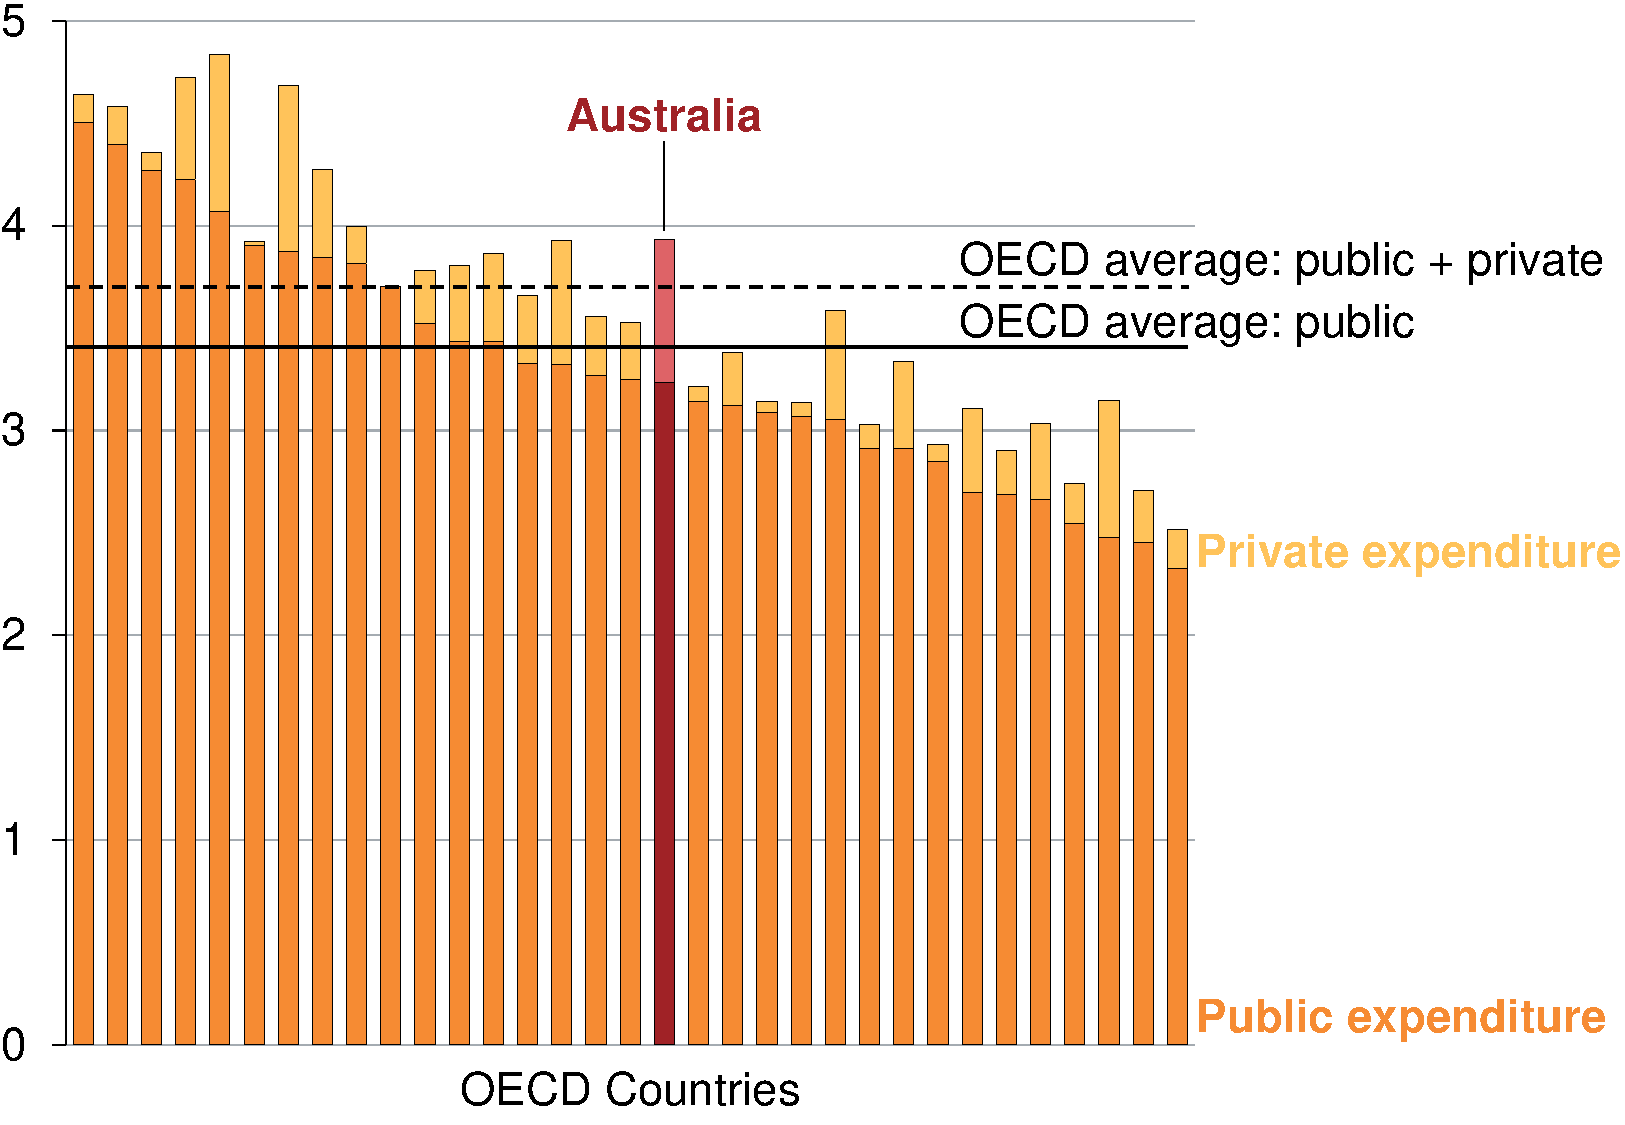
\includegraphics[page=1]{atlas/Charts.pdf}
\noteswithsources{This figure compares NEM capacity with peak demand since the NEM began. The intermittent component was calculated separately, with data for 2012-2017 only.}{Grattan analysis of \textcites{AER2017GenerationCapacityPeakDemand}{AEMO2017GenerationInfoJune}}
}{
\caption{Wholesale electricity prices have increased and are expected to remain above historic levels}\label{fig:wholesale-prices-have-increased}
\units{Price per megawatt hour}
\includegraphics[page=2]{atlas/Charts.pdf}
\noteswithsources{Solid lines indicate annual average wholesale prices (volume-weighted) since the NEM began. Dotted lines indicate average prices for quarterly base contracts for the next three financial years, as at the end of 2016-17. Note that contract prices tend to drop off over time because there is less demand over a year ahead.}{Grattan analysis of \textcites{AER2017AnnualVWASpotPrice}{AER2017BaseFuturesPrices}}
}

\begin{table}[t]
\caption{Short and long-term risks projected for the NEM}\label{tbl:projected-risks-for-the-NEM}
\begin{tabularx}{\linewidth}{XXR}
%
\toprule
\textbf{Region}                           & \textbf{2-year outlook}                              & \textbf{10-year outlook} \\
\midrule
South Australia & No shortfall with emergency measures & No shortfall but some risk in 2019-20 \& 2024-25\\
Victoria & No shortfall with emergency measures & No shortfall but some risk in all years\\
New South Wales & No shortfall & No shortfall but some risk from 2022-23 \\
Queensland & No shortfall & No shortfall\\
Tasmania & No shortfall & No shortfall\\
\bottomrule
\end{tabularx}
\noteswithsources{Emergency measures have been introduced for the 2017-18 summer to manage projected supply shortfalls in South Australia and Victoria, including bringing back mothballed capacity, new large-scale batteries and back-up diesel generation. `Some risk' refers to some expected unsupplied energy; `shortfall' refers to enough unsupplied energy to breach the NEM's reliability standard. The 2-year outlook is the June 2017 Energy Supply Outlook; the 10-year outlook is the Energy Statement of Opportunities September 2017 forecast.}{\textcites{AEMO2017ESO}{AEMO2017ESOO}}
\end{table}


\textbf{Resource adequacy} describes whether the system has \emph{sufficient} generation capacity and capabilities to meet demand for electricity over time. The challenge is to ensure enough generation is built (in terms of volume) and that the generation mix has the capabilities required to meet system needs (such as the ability to ramp up quickly, keep the system balanced, and minimise pollution).%
\footcite{Simshauser2010ResourceAdequacy}
New generation can take several years to build, so investment decisions must be \emph{timely} to meet changes in demand and supply. An effective market provides clear, timely price signals for investment and divestment. \Vref{fig:resource-adequacy-is-the-focus-of-this-report} illustrates how resource adequacy relates to the broader terms `reliability' and `security'.

\begin{figureTop}
\caption{This report focuses on resource adequacy}\label{fig:resource-adequacy-is-the-focus-of-this-report}
\units{}
\includegraphics[page=3]{atlas/Charts.pdf}
\notewithsources{Network capacity is not discussed in this report but is another component of resource adequacy}{\textcites{Simshauser2010ResourceAdequacy}{AEMC2016SSMFRInterim}}
\end{figureTop}

The market in 2017 is signalling for new investment, with tight supply, expected future closures, and high current and future prices. Yet no significant investment in firm capacity is evident (see \Vref{fig:investment-pipeline-is-predominantly-wind-and-solar}); there has been no new large-scale firm capacity in the NEM since 2012. New gas projects have stalled and investors do not see a future for new coal generation.%
\footcite{AEC2017CoalInTheNEM}
Investment in wind and solar has been strong in recent years, supported by the Renewable Energy Target (RET), but supply to balance wind and solar will be needed.

\begin{figureTop}
\caption{The investment pipeline is dominated by wind and solar}\label{fig:investment-pipeline-is-predominantly-wind-and-solar}
\units{Gigawatts of potential new generation capacity by fuel type and region}
\includegraphics[page=4]{atlas/Charts.pdf}
\noteswithsource{Potential new generation projects as at 5 June 2017. Proposed projects are those that have been publicly announced and may have completed initial feasibility studies, but have not yet received a Final Investment Decision (FID). Projects at the Committed stage of development have received a FID and have either started, or are expected to start construction. Rooftop solar PV installations are not included. Hydro and biomass are not included (because they are only a very small share of proposed projects).}{\textcite{AEMO2017GenerationInfoJune}}
\end{figureTop}

In this messy environment, governments have shown an appetite to invest in generation and storage themselves. The South Australian Government has announced plans to build a new gas-fired generator to provide power in emergencies.%
\footcite{SAGovt2017SAPlan}
The Federal Government has announced feasibility studies for major expansions of the Snowy and Tasmanian hydro schemes.%
\footcites{Massola2017SnowyHydroAnnouncement}{Turnbull2017TassieHydro}
Some Coalition MPs are arguing the Federal Government should build new coal-fired generation in Queensland.%
\footcite{Crowe2017CoalitionNewCoal}
The ACT Government has contracted for new renewable generation, and similar schemes are commencing in Victoria and Queensland. These interventions may undermine the operation of the NEM and deter private investors.%
\footcite{WoodBlowers-2017-Powering-Through}

It would be more efficient if private investors responded to market signals by building new generation (discussed further in \Chapref{chap:governments-may-intervene-regardless}). AGL's recent announcement that it will build a new gas generator in South Australia is a positive sign, although this is intended to replace existing gas generation rather than add to the total mix.%
\footcite{ABC2017AGLnewpowerstation}

\section{Policy stability is critical to resource adequacy}\label{sec:policy-stability-critical-to-resource-adequacy}
Investment decisions for new generation require a degree of predictability about future market conditions. Yet stability and predictability in energy and climate change policy has been lacking over the past decade. In submissions to the Finkel Review, the three largest electricity businesses in Australia -- AGL, Energy Australia and Origin -- cited climate change policy uncertainty as a major barrier to investment in new and existing generation. As Energy Australia noted:

\emph{`Even an astutely designed policy with relatively strong incentives for change will struggle to catalyse the required investment unless it is perceived by investors to be politically secure and robust at the outset.'}%
\footcite{EA2017FinkelSubmission}

A stable policy environment is a necessary condition for new investment.%
\footcites{WoodBlowers-2017-Powering-Through}{WoodBlowers-2016-Keeping-the-lights-on-SA}
Without policy stability, it is hard to see any circumstances under which the private sector will build enough generation.

\section{Finkel's blueprint could provide policy stability}\label{sec:finkel-review-focused-on-security-and-reliability}
After the September 2016 statewide blackout in South Australia, the COAG Energy Council (made up of Commonwealth, state and territory energy ministers) commissioned Alan Finkel to produce a blueprint for security and reliability in the NEM\@.

The Finkel blueprint, delivered in June 2017, lays out an `orderly transition' plan to give the market greater certainty on how emissions will be cut over time, and how the entry of new technologies and exit of old power stations will be managed.

The `orderly transition' plan includes:
\begin{itemize}
    \item An emissions reduction trajectory for the NEM that will `set expectations to guide investment decisions in the electricity sector';
    \item A Clean Energy Target (CET) that will cut emissions in a similar way to the existing RET, except it subsidises a range of cleaner energy technologies, not just renewables; and
    \item A requirement that all large generators provide at least three years' notice prior to closure.
\end{itemize}

Industry and consumers alike have widely supported the Finkel blueprint. But the package will only deliver policy stability if it is supported by the Commonwealth, all states, and all major political parties. The COAG Energy Council has accepted 49 of Finkel's 50 recommendations, but on the key recommendation of a CET there is, as yet, no agreement.%
\footcite{COAGEC2017JulyCommunique}


\section{Beyond Finkel}\label{sec:beyond-finkel}
While policy stability is a necessary condition to ensure resource adequacy, it may not be sufficient. The NEM is an \textbf{energy-only market}, meaning that generators are only paid for the energy they produce to meet demand.%
\footnote{Generators receive revenue through the wholesale market for the energy they produce. They also receive revenue through contract markets that are directly linked to the wholesale market, and through provision of ancillary services to help keep the system in balance (but ancillary services are usually only a small part of a generator's income).}
The term `energy-only' is used in contrast to markets that pay for both energy produced and generation capacity (whether or not it is needed).

The resource adequacy of energy-only markets such as the NEM has long been questioned and debated.%
\footcites{deVries2003InstabilityOfEOM}{hogan2005energy}{Joskow2006CompetitiveElectricityMarkets}{Joskow2008CapacityPayments}{Simshauser2008CapacityPayments}{Simshauser2010ResourceAdequacy}{Cramton2013CapacityMarketFundamentals}{Riesz2013CapacityMarket}{Hirth2014EnergyOnlyVsCapacity}{NewberyGrubb2014SecurityOfSupply}{Oxford2016ElectricityMarketsBroken}
Even Finkel argued that: \emph{`existing wholesale and contract market investment signals alone are no longer a suitably dependable mechanism to ensure the reliability of the NEM'}.%
\footcite[][83]{Finkel2017ReviewFinal}
However, in light of more urgent priorities, he did not recommend additional investment signals such as introducing a market for capacity.

AEMO's recent advice to the Federal Government on dispatchable capability argued in a similar vein that: \emph{`the current market design is unlikely to provide adequate and sustained signals to the market to incentivise development of new flexible dispatchable resources \dots{} over the medium and long-term.'}%
\footcite{AEMO2017AdviceDispatchableCapacity}
AEMO recommended a new long-term mechanism be developed.

This report focuses on whether the NEM can deliver resource adequacy in its current form (with the Finkel blueprint enhancements), or whether an additional mechanism is needed to ensure appropriate investment in future generation capacity.

We first explain how the market currently works and assess its performance to date (\Chapref{chap:how-the-market-incentivises-new-investment}). We then discuss new risks to resource adequacy that may arise from an energy market in transition (\Chapref{chap:why-the-NEM-might-not-work-in-future}).

The NEM has a strong record, and current risks to supply are manageable. But these emerging risks will make it more difficult to ensure adequate capacity in future. Given this uncertainty, Australia should start to prepare now for the possibility that an additional mechanism will be needed to ensure sufficient and appropriate generation and storage is built.

Recent events have shown that governments will intervene if the market is not seen to be delivering a dependable supply of electricity. But governments should not rush in, in case they make matters worse (\Chapref{chap:governments-may-intervene-regardless}).

There are several possible mechanisms to ensure resource adequacy (\Chapref{chap:what-are-the-options}). If a mechanism is needed, then preference should be given to one that maintains competitive pressure on market participants to build cheaper, cleaner and more reliable generation. Our conclusion is that private investors need to respond soon, and in the meantime, policy makers should begin preliminary design work and monitor the market closely (\Chapref{chap:what-governments-should-do}).



\chapter{The NEM has worked well so far}\label{chap:how-the-market-incentivises-new-investment}
In the NEM, generators are scheduled to dispatch electricity and are paid for the energy they supply. Retailers and large industrial consumers buy electricity through this market. All parties also contract with each other to manage their risk in the wholesale market. For the NEM to be sustainable, revenue from its wholesale and derivative contract markets must cover generators' full costs. The RET provides an additional revenue stream for renewable energy, independent of the wholesale and contract markets.

The NEM has worked well for almost 20 years but it now faces new challenges. The tightening of supply, policy uncertainty, and the increasing share of intermittent renewable generation (which has a different cost structure to traditional generation) will test the market.

\section{How generators make money in the NEM}\label{sec:how-generators-make-money-in-the-NEM}
Generators bid into the market to provide electricity for each five-minute interval of every day. AEMO ranks all bids in order from cheapest to most expensive (the `bid stack') and dispatches the cheapest set of bids that meets the needs of the system. The price paid to all generators dispatched is the bid of the last generator needed (see \Vref{fig:scheduling-of-NEM-generators}).

\begin{figure}
\caption{An example of the `bid stack' to determine dispatch and price}\label{fig:scheduling-of-NEM-generators}
\units{Output dispatched to meet 1000 megawatts of demand}
\includegraphics[page=5]{atlas/Charts.pdf}
\notewithsource{In this example, the bid of Generator 5 (\$50 per MWh) sets the price paid to all five generators needed to meet demand. Generator 6 is not required, so does not receive any payment.}{Reproduced from \textcite[][11]{AEMO2010NEMExplainer}}
\end{figure}

The incentive is for generators to bid at their marginal cost -- the cost of producing an extra unit of electricity. If they bid a higher price they risk not being dispatched and therefore not receiving any revenue. If they bid a lower price they could lose money on the electricity they produce.

When a generator with high marginal costs sets the price, all other generators benefit from additional revenue. They get a price for electricity that is greater than their marginal cost, allowing them to recover some of their fixed costs.

But if every generator bids into the market at their marginal cost there is a problem: when does the generator with the highest marginal cost recoup their fixed costs? High marginal-cost generators rely on scarcity pricing -- infrequent periods of very tight supply, when they can set the price high enough to recover their fixed costs.%
\footnote{Scarcity pricing is not the same as exercising market power. Scarcity pricing only occurs during tight supply when the marginal generator is the final generator available to be dispatched. Exercising market power means artificially increasing prices through behaviour to increase revenue.}
All generators benefit from additional revenue during scarcity periods.

Prices in the wholesale electricity market are volatile, so market participants manage their exposure through vertical integration or through contracting with each other. High prices pose a risk for retailers, while periods of low or highly unpredictable prices pose a risk for generators. Contracts are typically based on an average price, reducing the risks for both parties. This is known as `hedging'.

All electricity is traded through the wholesale market even though at any given time, most of it is under private contract.%
\footnote{90-100 per cent of a typical retailer's load is under contract (\textcite{MEI2016ContractPosition}).}
The price agreed in the contract is the price paid for electricity by end consumers, but contracts remain linked to the wholesale `spot' price.

For example, under a `swap' contract, a retailer can agree to buy electricity from a generator for an expected average of the spot price over a period of time. Under a `cap' contract, retailers pay generators a fixed price to reduce their exposure to high spot prices (usually over \$300 per megawatt hour). If the high price occurs, the generator effectively pays the difference between the actual spot price and the agreed cap price on behalf of the retailer. When wholesale prices rise, the value of swap contracts will increase too, and when wholesale prices are frequently very high, the value of cap contracts increases. The wholesale and contract markets are therefore linked, and both are important to how generators make money in the NEM\@.


\section{High prices and contracts encourage new investment}\label{sec:scarcity-pricing-encourages-new-investment}
Energy-only markets rely on high prices during times of scarcity to prompt new investment (or to bring back mothballed capacity).%
\footcite{hogan2005energy}
The size and duration of high prices provides a signal, not just for more supply, but also for the kind of generation that is most needed in the market.%
\footnote{\eg{} If price peaks are brief but very high, more flexible generation might be needed that can be switched on during peak periods. Alternatively, if prices are up throughout the day, a low-cost baseload generator may be needed.}

While high prices provide the signal, contracts provide the means. A contract offers a guaranteed revenue stream that helps in accessing loans and securing the finance required to build a new generator. `Futures' trading on the ASX is available up to four years ahead of delivery, and private `over the counter' (OTC) bilateral contracts can be much longer.%
\footnote{Although because these deals are made privately, there is no real visibility of contract volumes, terms, or length.}

Usually a retailer will have almost all their customer load under contract for the year ahead, but very little under contract four-to-five years out (see \Vref{fig:most-demand-is-under-contract}).
This means new and existing generators may not have security of revenue in the long term. Unless generators can secure a long-term contract for supply (with a retailer or a large industrial customer), they will be reliant on wholesale prices staying high enough over time to ensure future short-term contracts continue to cover their costs.

\begin{figureTop}
\caption{Most demand is under contract in the short-term}\label{fig:most-demand-is-under-contract}
\units{Per cent of load hedged for a typical retailer}
\includegraphics[page=6]{atlas/Charts.pdf}
\notewithsource{J\@.P\@. Morgan estimates of a typical hedge book profile, based on company data.}{Reproduced from \textcite{MEI2016ContractPosition}.}
\end{figureTop}

\section{The NEM has delivered sufficient capacity}\label{sec:the-NEM-has-delivered-investment-in-the-past}
The success of the NEM in delivering resource adequacy over the past two decades suggests that energy-only markets can work.

Only twice has there been insufficient capacity in the market to meet the reliability standard:%
\footnote{The reliability standard sets the expectation that demand will be met 99.998 per cent of the time in each region in the NEM\@. In practice this means that electricity supply can be at risk for only 11 minutes per year per region, on average, usually at times of peak demand. This standard is set by the Australian Energy Market Commission's Reliability Panel to guide investments in generation and transmission to meet the standard (\textcite{AEMC2017ReliabilityStandardReview}).}
in Victoria and South Australia in January 2009, during the height of a heatwave and drought that contributed to the Black Saturday bushfires in Victoria.%
\footnote{Other blackouts have occurred, but most blackouts arise because something in the system breaks rather than because of insufficient generation capacity (\textcite{AEMO2017FinkelSubmission}).}

%\begin{figure}
%\caption{Only two reliability breaches in the history of the NEM}\label{fig:Only-two-reliability-breaches-in-the-history-of-the-NEM}
%\units{Unsupplied energy (per cent of regional native consumption)}
%\includegraphics[page=7]{atlas/Charts.pdf}
%\noteswithsource{There may have been breaches of the reliability standard in the most recent year, 2016-17, but this will not be reported until March 2018.}{Grattan analysis of \textcite{AEMC2017AnnualMarketPerformance2016} and historical data from \textcites{AEMC2016AnnualMarketPerformance2015}{AEMC2014AnnualMarketPerformance2013}}
%\end{figure}

In each year of the past decade there have typically been only 10-20 occasions where back-up was \emph{not} available, had it been needed.
However, in 2016-17 this jumped to around 50 occasions, indicating that supply is much tighter since the retirement of Northern power station in May 2016 and Hazelwood in March 2017.%
\footcite{AEMC2017ReliabilityFrameworksIssuesPaper}

Many new generators have been built in the past 20 years, while others have exited the market (see \Vref{fig:substantial-investment-and-divestment-in-generation-over-time}). This seems to suggest that an energy-only market can provide the right signals to drive the investment that is needed, but as the next section shows, government policy settings have been an important influence.

\begin{figureTop}
\caption{There has been substantial investment and divestment in generation since the NEM began}\label{fig:substantial-investment-and-divestment-in-generation-over-time}
\units{Annual change in generation capacity, gigawatts}
\includegraphics[page=8]{atlas/Charts.pdf}
\notewithsources{Retirements exclude mothballed plants that are not in use bus can be brought back into use.}{The Australian Energy Regulator (AER) provided data up to 2015-16 as per \textcite{AER2017StateofEnergyMarket}; 2016-17 data comes from AEMO generation information as at 5 June 2017 (\textcite{AEMO2017GenerationInfoJune}).}
\end{figureTop}

\section{Policy settings have been important to investment}\label{sec:government-policy-settings-important-to-investment}

Since market liberalisation in the late 1990s, most new capacity has come from the private sector.%
\footnote{\textcite{Simshauser2009ToxicDebt}. Note until the early 1990s, power stations were financed by loans either backed or issued by state governments. All government-owned power stations in Victoria and South Australia were privatised by the late 1990s, and most NEM jurisdictions had surplus capacity when the NEM was created in 1998. Queensland was a notable exception -- market conditions at the time of liberalisation favoured investment in baseload generation and led to excess entry into the market, see \textcite{Simshauser2006StructuralFaultsEOM}.}
But government policy settings have created favourable conditions for a large share of private investment, in three ways (see \Vref{fig:public-private-investment-in-generation}).

\begin{figureTop}
\caption{There has been a mix of public and private investment in new large-scale generation}\label{fig:public-private-investment-in-generation}
\units{Total investment in generation capacity, gigawatts, 1999-2016}
\includegraphics[page=17]{atlas/Charts.pdf}
\noteswithsources{Coal, gas, wind and solar represent 95 per cent of large-scale generation investment in the NEM since 1998. The other 5 per cent includes hydro, landfill gas and diesel, among other things. The Queensland Government's Gas Scheme encouraged private investment in 2GW of new gas. The `Government' column includes 1.3GW of coal entered into as a 50/50 public-private joint venture. Most large-scale wind and solar generation is privately-owned, but subsidised under the Federal Government's Renewable Energy Target.}{Grattan analysis of AER data of new investment by fuel type (\textcite{AER2017StateofEnergyMarket}), AEMO generation information as at 5 June 2017 (\textcite{AEMO2017GenerationInfoJune}), and \textcite{Simshauser2008CapacityPayments}.}
\end{figureTop}

First, two major coal-fired power stations built in the early 2000s were 50/50 joint ventures between government-owned and private companies.

Second, the Queensland Government encouraged significant investment in new gas generation from 2005 to 2013 by requiring electricity retailers to obtain 15 per cent of electricity sold or used in Queensland from power generated using natural gas.%
\footcite{Gibson2013QLDGasScheme}

Third, renewable energy receives additional revenue under the RET, so while the private sector has been investing in large-scale renewable generation, particularly wind, these investments are subsidised. And some have also been supported by government grants through the Australian Renewable Energy Agency (ARENA) and long-term contracts under the ACT Government's reverse auction scheme.

It is unclear what policy settings (if any) will drive new investment in the decades to come. And there are other uncertainties:
\begin{itemize}
    \item Rising demand has been an important driver of investment in the past, but the demand outlook is now flat;
    \item An ageing generation fleet means power station closures are on the horizon and the exact timing of these retirements may not always be predictable; and
    \item The increasing penetration of intermittent renewable generation creates new risks for investors and consumers, as the next chapter will show.
\end{itemize}



\chapter{Why the NEM might not work in future }\label{chap:why-the-NEM-might-not-work-in-future}
The rise of intermittent renewable energy raises new questions about the effectiveness of investment signals in the NEM\@. Wind and solar generators have different cost structures and availability that challenge the existing market. All generators -- including wind and solar -- may struggle to recover their full costs in the NEM as the proportion of intermittent renewables grows.

Prices are likely to be more volatile, with more low prices when wind and solar energy are available and more high prices when they are not. Extreme price volatility creates problems for an energy-only market. Governments would have to accept the need for very high prices in times of short supply. Market participants would have to increase both short-term hedging activity to manage risk, and longer-term contracting to secure investment. And households and businesses would also need to be more flexible in their electricity use when supply is tight. It will not be easy to meet all three conditions.

\section{It will be harder to recoup fixed costs in a zero-marginal-cost world}\label{sec:it-will-be-harder-to-recoup-fixed-costs-in-a-zero-marginal-cost-world}

The NEM was not designed with the rapid rise of wind and solar generation in mind. Yet renewables now represent a major share of generation in some regions, particularly South Australia. They have a different cost structure. Wind and solar have high capital costs but effectively zero marginal costs; once the facility is built, the energy produced is essentially free.

Given generators have an incentive to bid their marginal cost, when there is more zero-marginal-cost generation in the market, there are more periods when the wholesale price is very low or zero. During these periods, all generators -- including renewables -- will struggle to recover their fixed costs.%
\footcite{Riesz2013CapacityMarket}
At present, low prices are less of a problem for renewable generators because they receive revenue through the RET when they generate.%
\footnote{Also some state governments are providing -- or proposing to provide -- contracts to renewables that guarantee revenue, regardless of the wholesale market price.}
But the RET plateaus after 2020 (although the CET will help, if it comes into effect).%
\footnote{The RET peaks in 2020, but certificates to meet the 2020 target must continue to be surrendered until 2030 when the scheme will fully close.}

The result of this dynamic is shown in \Vref{fig:hypothetical-example-of-intermittent-renewables-price-volatility}. As intermittent zero-marginal-cost generation is added, generators can only recover their costs if there are more high price events (and/or \emph{higher} high price events) to counteract times when there are low, or even negative, prices. This will lead to greater price volatility.

\begin{figureTop}
\caption{More reliance on intermittent renewables means more price volatility}\label{fig:hypothetical-example-of-intermittent-renewables-price-volatility}
\units{}
\includegraphics[page=9]{atlas/Charts.pdf}
\noteswithsource{LRMC = long-run marginal cost; SRMC = short-run marginal cost}{Grattan analysis}
\end{figureTop}

South Australia, where wind accounts for more than 40 per cent of the electricity generated, illustrates this dynamic. Very low and very high prices are far more frequent there than in states with less intermittent generation (see \Vref{fig:price-volatility-is-increasing-in-South-Australia}).

\begin{figureTop}
\caption{Price volatility is increasing in South Australia}\label{fig:price-volatility-is-increasing-in-South-Australia}
\units{Frequency of prices below \$0 or above \$300 per megawatt hour by financial year}
\includegraphics[page=10]{atlas/Charts.pdf}
\source{Grattan analysis of price and demand data, 2010-11 to 2016-17, requested from AEMO\@.}
\end{figureTop}

Price volatility is an important feature of an efficient market, because high prices provide an incentive for new investment. But extreme price volatility increases the risks and associated costs for all market participants. And these risks and costs need to be managed if new generation is to be built. Increased price volatility could be challenging for three reasons:
\begin{enumerate}
    \item Higher and more frequent price spikes may prove too risky for investors, retailers, consumers and/or governments;
    \item There may be too few contracting opportunities to manage risk and bring on new supply; and/or
    \item Demand may prove to be insufficiently flexible to ensure resource adequacy.
\end{enumerate}

\section{High prices can mean unacceptable risks}\label{sec:high-prices-mean-unacceptable-risks}
The price volatility created by high proportions of zero-marginal-cost electricity may be unacceptable to investors, retailers, consumers, and governments.%
\footcites{Nelson2016NewNEM}{AESO2016AlbertaMarketReform}
High volatility in spot market prices and therefore in revenue will make financiers nervous if a large proportion of a generators' revenue relies on unpredictable periods of high pricing.

Wholesale electricity markets usually have imposed price floors and caps to protect participants against extreme risks. The Market Price Cap (MPC) is the key regulatory mechanism designed to ensure that prices can get high enough to attract new investment, but not so high as to hurt consumers (through abuse of monopoly market power in times of scarcity).%
\footnote{The MPC is set by the AEMC's Reliability Panel, at a level deemed sufficient to deliver the investment in generation capacity needed to ensure the NEM's `reliability standard' is met (\textcite{AEMC2017ReliabilityStandardReview}).}

If the price cap is set too low, new investment may be deterred because there may not be sufficient revenue in the market for generators to recover their fixed costs. The MPC in Australia, now \$14,200 per megawatt hour, is considered high by international standards (see \Vref{tbl:price-caps-in-energy-only-markets}).%
\footcite{CIGRE2016CapacityMechanisms}
A high MPC means greater price volatility.

\begin{table}
\caption{Price caps in energy-only markets}\label{tbl:price-caps-in-energy-only-markets}
\begin{tabularx}{\linewidth}{XXR}
%
\toprule
\textbf{Jurisdiction}                           & \textbf{Market price cap (\$AUD/MWh)} \\
\midrule
Alberta & \$1,010\\
Singapore & \$4,185\\
North-western Europe & \$4,410\\
Texas & \$11,340\\
\rowcolor{Gray}
Australia & \$14,200\\
New Zealand & \$9,400-\$18,800*\\
\bottomrule
\end{tabularx}
\noteswithsource{*New Zealand's scarcity pricing range only applies when load-shedding has been triggered because of a supply shortfall. All price caps are set relative to reliability standards, which differ between electricity systems.}{Grattan analysis of market operator information}
\end{table}

As the share of intermittent renewables in the market increases, prices may need to go even higher and the price cap may need to be increased.
A 2016 study modelled an extreme scenario of 100 per cent renewables and no demand response. It estimated a price cap of between \$60,000 to \$80,000 per megawatt hour would be required to ensure sufficient revenue in the market.%
\footcite{Riesz2016MPCwithRenewables}

Any proposal to raise the price cap substantially is likely to meet community and political resistance. Even though a higher price cap may ultimately be best for consumers,%
\footnote{Compared to a new mechanism to compensate generators in addition to the energy-only market.}
politicians are likely to intervene, as demonstrated by their reaction to high price events in July 2016 and since.%
\footcites{WoodBlowers-2017-Powering-Through}{WoodBlowers-2016-Keeping-the-lights-on-SA}

That would be dangerous. If politicians prevent the price cap from increasing sufficiently, they will create a \textbf{`missing money problem'}: insufficient revenue available in the market leading to under-recovery of fixed costs and under-investment.%
\footcites{Joskow2006CompetitiveElectricityMarkets}{Joskow2008CapacityPayments}
At this point there would be a resource adequacy problem, unless governments reform the market or raise the price cap.

\section{There may not be enough contracting opportunities}\label{sec:are-contracting-opportunities-sufficient}
As price volatility increases, the need to hedge risk and the cost of hedging will also increase. A robust energy-only market encourages a variety of voluntary contracts to reflect the different risk preferences of market participants.%
\footcites[][8]{hogan2005energy}[][3]{Yarrow2014Bidding}
Different contract lengths suit different parties. If there is not enough risk trading (`liquidity') to suit all parties, this could discourage investment, posing a threat to the energy-only market.%
\footnote{\eg{} \textcite{Gauthier2017TheNeedForLongtermContracts} and \textcite[][224]{helm2017burnout}: \emph{`energy-only markets have failed to provide deep, liquid and transparent trading to hedge risk'}.}

Opportunities to hedge risk in the short-term are particularly critical for small retailers.%
\footnote{Insufficient opportunities to hedge led to a small retailer in NSW going bust in 2007 when faced with spot market payments that exceeded its financial capacity. Queensland experienced times of insufficient hedging between 2000-2005, but because the retailers were state-owned, they had the backing of the Queensland Treasury and were able to manage, see \textcite[][14]{Simshauser2010EntryCostShock}.}
Long-term (5 years +) contracting opportunities are particularly important for new generation, given the time it takes to build new generation and then recoup those costs in the market over time. New, fixed-cost generation and storage may look to sign long-term contracts before commitment.

But the market may not provide the conditions for sufficient contracting due to:
\begin{itemize}
    \item Increased vertical integration limiting the parties available to enter into contracts;
    \item Increased penetration of intermittent generators that do not currently provide full risk coverage;
    \item Customer switching limiting the ability of retailers to enter into long-term contracts; and
    \item Policy uncertainty making parties on both sides reluctant to enter into long-term contracts.
\end{itemize}

If businesses need to reduce their risk in the market, rather than contract, they may opt to purchase their own generation. Businesses that operate in both the retail and wholesale markets are `vertically integrated': the retail side of the business can protect the generation side and vice versa. Some people argue that `the days of the retail only business are numbered'.%
\footcites{Potter2017Powershop}{Simshauser2017IntermittentGeneration}
Vertically integrated `gentailers' effectively hedge with themselves (at least in part), reducing the availability of contracts for other market participants.

Intermittent renewable generators cannot provide retailers with full risk coverage because they cannot be sure they will be able to supply energy during high price events. Given that investment in intermittent renewables is usually backed by long-term power purchase agreements (PPAs) under the RET, additional hedging contracts are not needed. Without the RET, new intermittent renewables might choose to have some firm back-up capacity, so they can participate more fully in the contracts market.%
\footnote{Finkel's `Generator Reliability Obligation' should partially remedy this because it will require new intermittent generators in regions that already have a high share of intermittent generation to have some firm back-up supply. Those generators may therefore be able to enter contracts.}
The low hedging activity in South Australia may be explained by the vertical integration of the largest market participants, combined with the rise of intermittent renewables (see \Vref{fig:trading-activity-lower-in-South-Australia-and-may-be-in-decline-across-the-board}).%
\footnote{The most recent data show the share of trading between regions to be roughly one third each for Victoria, Queensland and NSW, while South Australia represented only 1 per cent of traded volume (\textcite[][13]{AFMA2016AFMR}). Energy users in South Australia also report problems with contract availability (\textcite[][81]{Finkel2017ReviewFinal}).}

While retailers are likely to need short-term hedging contracts, they may be reluctant to enter into long-term contracts. In a recent survey, some retailers commented that their contracts with generators have shortened because their large-customer contracts are shortening.%
\footcite[][60]{AEMC2017RetailCompReview}
Customers are requesting shorter contracts because they expect wholesale prices will decrease soon.%
\footcite[][60]{AEMC2017RetailCompReview}
A separate analysis shows the length of commercial and industrial consumers' retail contracts has declined over the past decade and is now less than two years on average.%
\footcite{Simshauser2017IntermittentGeneration}
The market has a problem if consumers want shorter contracts in response to high prices, but long-term contracts are needed to bring in new supply.

\begin{figureTop}
\caption{Trading activity is lower in South Australia and may be in decline across the board}\label{fig:trading-activity-lower-in-South-Australia-and-may-be-in-decline-across-the-board}
\units{Volume of electricity traded as a share of regional consumption}
\includegraphics[page=11]{atlas/Charts.pdf}
\noteswithsources{Data only available up to 2014-15. AFMA reporting changed from 2015-16, with previous data based on a survey that has now been discontinued.}{Grattan analysis of \textcites{AFMA2015AFMR}{AER2017RegionalDemand}.}
\end{figureTop}

A lack of long-term contracting may be limiting new investment in the NEM\@. Most electricity is contracted for less than one year (\Vref{fig:less-than-half-of-contracting-activity-is-longer-than-a-year}).

\begin{figureTop}
\caption{Most electricity is contracted for less than a year}\label{fig:less-than-half-of-contracting-activity-is-longer-than-a-year}
\units{Per cent of megawatt hours under contracts of 1 year or less}
\includegraphics[page=12]{atlas/Charts.pdf}
\noteswithsource{Data only available up to 2014-15. AFMA reporting changed in 2016.}{\textcite{AFMA2015AFMR}}
\end{figureTop}

Policy uncertainty also reduces the ability of parties to enter into long-term contracts. The RET encouraged retailers to enter into PPAs with new renewable energy generators.%
\footcite{anderson2007forwardcontracts}
But the RET incentive is now drying up and policy uncertainty is reducing companies' willingness to sign long-term PPAs.%
\footcites[][20]{ChiefEcon2015ElectricityGenProjects}{Abernethy2017PPAs}

Government contracts have underpinned recent investments in renewable energy and storage.%
\footnote{The ACT Government has backed a series of renewable energy investments through 20-year contracts (\textcite{ACTrenewablesauctions2016}). The South Australian Government recently announced a new solar thermal power plant in Port Augusta backed by a 20-year government contract (\textcite{ABC2017SolarThermalPortAugusta}) and has also awarded a tender to Tesla to build a large-scale battery facility (\textcite{Harmsen2017TeslaBatterySA}). And the Victorian and Queensland Governments have just announced tenders for large-scale renewable generation and storage (\textcites{VICrenewablesauctions2017}{QLDrenewablesauctions2017}).}
The only recent private contract to increase supply was the deal struck between Origin Energy and Engie to bring Pelican Point power station in South Australia back online.%
\footcite{AFR2017PelicanPointGasPrice}

It is not clear if incentives are sufficient for retailers and large consumers to enter into long-term contracts with new generation. It is clear that climate change policy remains a major uncertainty for all players.%
\footcite{Simshauser2017IntermittentGeneration}
Price volatility may promote short-term trading, particularly cap contracts,%
\footnote{In a world of greater price volatility, we may see an increase in cap contracts. Under cap contracts, the retailer pays the generator a specified price to reduce the retailer's exposure to high price events (usually over \$300 per megawatt hour).}
but may deter parties from entering into long-term contracts because of uncertainty about future prices.

Overall, it is hard to tell if contracting is sufficient to enable new investment. The extent of long-term contracting is unclear because ASX products are only available up to three-to-four years ahead and there is no visibility of direct bilateral agreements.%
\footnote{AFMA has not published OTC contract volumes since 2014-15.}
The Finkel blueprint recommends monitoring the price and availability of long-term retail contracts in an annual \emph{Health of the NEM} report. This would enhance public knowledge of contracting behaviour in the energy sector.%
\footcite[][140--141]{Finkel2017ReviewFinal}

\section{Demand is largely inflexible}\label{sec:inflexible-demand}

Energy-only markets rely on having some flexible demand to manage price volatility and ensure resource adequacy.%
\footnote{\emph{`Suppose electricity markets did not suffer from demand-side flaws \dots{} then, the market would be perfectly reliable'} (\textcite{Cramton2013CapacityMarketFundamentals}).}
Large consumers can reduce their exposure to extreme prices by reducing their demand at peak times. With active `demand response', only those consumers that place a very high value on reliability are exposed to the high prices.%
\footnote{\textcite{Riesz2013CapacityMarket}: \emph{`[With demand-side participation] the aggregate reliability standard implied by the MPC can gradually apply to a diminishing proportion of the system. Eventually, with very comprehensive demand side participation, it may be possible to remove the need to apply a regulated MPC.'}}
Paying consumers to temporarily reduce demand during times of tight supply can reduce the total amount of generation that needs to be built, reducing system costs for everyone.

But most demand for electricity is currently inflexible.%
\footcites{AEMO2017ESOO}{CSIRO2015CostReflectivePricing}{fan2011price}{reiss2005household}
A lack of cost-reflective pricing means most consumers are shielded from the real costs associated with their patterns of electricity use. Few households have the interest or time to respond to real-time electricity price signals.%
\footcite{CSIRO2015CostReflectivePricing}
But there are signs of increasing responsiveness.

Public notification of a critical peak period during the February 2017 heatwave appears to have been effective in reducing electricity use.%
\footcite{OKane2017EnergySecurityTaskforceInitialReport}
And AEMO and ARENA are trialling a scheme in which consumers receive incentive payments to be on standby in emergencies or peak demand days. Those who reduce their electricity use temporarily, if called on by AEMO, will receive a further compensation payment.%
\footcite{AEMOARENA2017DemandTrial}

A more structural approach, where consumers' high-energy appliances are managed centrally in exchange for a reduced tariff, may be more attractive to consumers.%
\footcite{CSIRO2015CostReflectivePricing}
Such schemes should be more widely available, because without some flexible demand in the system it is hard for energy-only markets to ensure resource adequacy during rare and extreme demand peaks.

\section{Can the NEM survive the transition?}\label{sec:can-the-nem-survive-the-transition}
The NEM will be put to the test over the coming decade.

An increasing share of intermittent, zero-marginal-cost generation creates new risks in an energy-only market. There will be more periods of very low prices when zero-marginal-cost generation is available, and very high prices at other times when other generators attempt to recover their costs. This price volatility is necessary to avoid the `missing money problem', but the price volatility itself increases risks and costs for all market participants.

Price volatility will increase the need for hedging and bilateral contracts. In particular, long-term contracts will be needed to provide financial backing to new generation as spot price outcomes become less certain. At the moment, only governments are signing long-term contracts. An end to the decade-long instability in climate change policy would help enable market participants to do these deals themselves.

More contracting would ensure resource adequacy can be delivered within the existing market structure. But there are other uncertainties too. Retailers and large consumers may not be willing to enter into long-term contracts to bring in new supply, given uncertainty about their future electricity needs and cheaper technologies on the horizon.

For the energy-only market to deliver resource adequacy through the transition, Australian governments will need to allow the market price cap to increase, as required, and market participants will need to manage the associated risks and costs through contracting -- including providing the long-term contracts needed to back new generation. Market participants will also need to source more flexible demand, to reduce the total amount of generation that needs to be built and ensure resource adequacy during times of tight supply.

Market participants will have to respond in the next year or so to restore confidence in the existing market structure. With five years until the next major power station is expected to retire, there is still time.%
\footnote{At least 2,000 megawatts of coal-fired power in NSW is expected to be retired in 2022 when Liddell power station is due to shut.}

If these conditions cannot be met, then governments will need to find alternative mechanisms that ensure sufficient and appropriate generation is built. Early warning signs that the market may no longer be able to deliver new investment include a rising imbalance between exit and entry in the market, wholesale prices regularly hitting the price cap, demand inflexibility, and lack of availability of long-term contracts.

The next chapter warns governments against certain kinds of responses to supply risks. \Chapref{chap:what-are-the-options} assesses alternative market models that would ensure resource adequacy. The final chapter details what governments should do now.


\chapter{Governments might intervene regardless}\label{chap:governments-may-intervene-regardless}
More summers where supply is tight, and more projected shortages in electricity generation, may tempt politicians to conclude that the market is broken and intervene. Governments fear that if they do not act when there is sign of a shortfall in generation capacity, there will be widespread blackouts. But market participants may respond with new investment, demand-side measures may reduce peak demand, and/or the forecast itself may change before the shortfall eventuates. Even if a feared shortfall does eventuate, there are mechanisms available to prevent the worst from happening.

Nonetheless, governments and the public need greater assurance. A more robust and comprehensive monitoring of resource adequacy in the NEM is required, including a trigger point for intervention. If intervention is required, governments should not invest directly. Instead, intervention should be in the form of a market redesign, triggered by the Energy Security Board, not by governments.%
\footnote{The Energy Security Board (ESB) was established in August 2017 to provide whole of system oversight for energy security and reliability. The ESB comprises an independent Chair and Deputy Chair, plus the heads of the AEMC, Australian Energy Regulator and AEMO.}

Predictions of shortages in the medium-term have prompted other jurisdictions, including the UK and France, to redesign their electricity markets (see \Vref{box:why-other-countries-have-moved-away-from-energy-only-markets}).

\begin{bigbox*}{Why other countries have moved away from energy-only markets}{box:why-other-countries-have-moved-away-from-energy-only-markets}
\setlength{\parskip}{6pt}
\setlength{\intextsep}{6pt}
\begin{alphafootnotes}
In general, governments that have moved away from energy-only markets have done so not because the market has broken, but because they fear the market will break.%
\footcite{CIGRE2016CapacityMechanisms}
The main triggers have been the `missing money problem', a changing supply mix, and forecasts of potential shortages.

\textcolor{Orange}{Missing money and the changing supply mix}

The UK introduced a capacity market in 2014 as part of wider reforms to maintain reliability while decarbonising the UK's electricity supply. Older, polluting power stations were closing while demand increased.%
\footcites{Ofgem2017EMR}{DECC2014EMR}
A capacity market was introduced as an incentive for investment, specifically to counter the `missing money problem':
\emph{`There is a significant risk that the market will no longer deliver an adequate level of security of electricity supply as it has done historically, principally because potential revenues in the energy-only market may no longer incentivise sufficient investment in capacity.'}
\footcite[][1]{DECC2014EMRCapacityImpactAssessment}

It was estimated that the existing market price cap of £1,000 would need to be raised to £17,000 to avoid the `missing money problem'. This was considered unacceptably high and a capacity market was preferred because it is less risky for investors than scarcity pricing.%
\footcite[][59]{DECC2014EMRCapacityImpactAssessment}

Alberta also identified missing money and the changing supply mix as drivers of its 2016 decision to move away from an energy-only market. After interviewing investors and lenders, Alberta's market operator, AESO, concluded there may not be sufficient investment in non-renewable generation. AESO tested whether raising the market price cap from USD\$1,000 to \$5,000 would help, and concluded that although this would provide enough revenue, the price volatility would create unacceptable risk for consumers.%
\footcite{AESO2016AlbertaMarketReform}

\textcolor{Orange}{Forecasts of capacity shortages}

The UK and France cited looming shortages as a rationale for abandoning energy-only markets.

The UK concluded that in the absence of a capacity mechanism, shortfalls would begin within a decade. France introduced a capacity mechanism because medium-term forecasts showed shortfalls. Peak demand is growing much more quickly than average demand in France.

Texas considered introducing a capacity mechanism when forecasts showed shortfalls, but decided against when peak demand began to fall and new forecasts showed resource adequacy would be met, largely through existing supply.

Poland introduced a strategic reserve mechanism after forecasts showed short-term resource adequacy was at risk. But the shortages were caused in part by government regulation to decommission plants that did not meet environmental regulations, rather than the market failing to provide the necessary generation.%
\footcite{CIGRE2016CapacityMechanisms}

\end{alphafootnotes}
\end{bigbox*}

\section{Current forecasts are for industry, not governments}\label{sec:current-forecasts-for-industry-not-governments}
AEMO publishes an annual Electricity Statement of Opportunities (ESOO) that identifies potential capacity shortfalls over a 10-year period. The purpose of the document is to provide information to industry, not a trigger point for politicians to intervene.

The ESOO is quite variable (see \Vref{fig:resource-adequacy-projections-over-time}) -- one ESOO can show a shortfall is 10 years away and the next can show it is only two years away. This happens when a large amount of capacity is removed from the system, or when demand and weather forecasts change substantially. New generation can take years to build, so it is understandable that politicians may rush to intervene in this situation. However, there are many ways that market participants can respond that would be more efficient and effective.

In the past, when the ESOO has projected a shortfall, the market has responded or other circumstances have changed after the forecasts were issued such that additional supply was no longer needed. Expectations for demand may be revised down, a new generator may be built, or market participants might bring back mothballed generation capacity as a temporary measure to meet the shortfall.

The ESOO plays an important role in signalling the need for new investment or other actions from industry. But it does not provide governments and the public with reassurance about how shortfalls will be met.

\begin{figureTop}
\caption{Views about future shortages have changed very quickly}\label{fig:resource-adequacy-projections-over-time}
\units{Number of years until a potential shortfall, by year of forecast}
\includegraphics[page=13]{atlas/Charts.pdf}
\noteswithsources{Resource adequacy forecasts look up to 10 years ahead. A forecast identifies a potential shortfall if the supply-demand balance within a region is tight enough that the reliability standard can no longer be confidently met for that year. Emergency measures are in place to avoid projected shortfalls in the coming summer, and no shortfall is projected after 2017-18, see \Cref{tbl:projected-risks-for-the-NEM}. Note the 2016 forecast reflects the impact of Hazelwood's retirement.}{Grattan analysis of \textcites{AEMO2010ESOO}{AEMO2011ESOO}{AEMO2012ESOO}{AEMO2013ESOO}{AEMO2014ESOO}{AEMO2015ESOO}{AEMO2016ESOO}{AEMO2017ESOO}}
\end{figureTop}

\subsection{What a projected shortfall really means}\label{subsec:what-a-projected-shortfall-really-means}
The ESOO points to a potential shortfall when there is a risk that the NEM’s reliability standard will be breached. The reliability standard sets the expectation that demand will be met 99.998 per cent of the time, meaning that electricity supply can be at risk for only about 11 minutes per year per region, on average. The forecast identifies a potential shortfall if electricity supply in any region is at risk for longer than this. The impact may be very small or very large depending on the exact nature and length of a particular shortfall.

The likelihood of a shortfall actually eventuating is sensitive to many factors beyond the amount of generation available, including expectations for demand, temperatures and rainfall. Forecasts are appropriately conservative and may be revised down closer to the time.

Forecasts of potential shortfalls provide an important signal to investors to build new generation -- they do not imply a market failure if there is time for investors and/or other market participants to respond.

\subsection{The consequences if a shortfall eventuates}\label{subsec:consequences-if-a-shortfall-eventuates}
Even if a feared shortfall does eventuate, the consequences, while uncomfortable, will not be as disastrous as the 2016 state-wide blackout in South Australia.

First, the market operator has powers to bring on temporary supply or demand response, if available, to prevent a supply shortfall.%
\footnote{Under the Reliability and Emergency Reserve Trader (RERT) mechanism, AEMO can contract with generators and demand-response providers to be available if it considers a capacity shortage to be imminent. See \textcite{WoodBlowers-2017-Powering-Through}.}
For example, AEMO is using its powers this summer to procure up to 1,000 megawatts of additional generation capacity and demand response.%
\footcite{AEMO2017AdviceDispatchableCapacity}

Second, if that is not sufficient, temporary power restrictions may be imposed on some consumers, where their power is reduced or switched off for half an hour or so (`load shedding').

While no doubt inconvenient, this is a controlled situation. The blackout last September, driven by extreme weather conditions, was not.

\section{Governments need a more robust monitoring framework}\label{sec:governments-need-a-more-robust-monitoring-framework}
The ESOO is not sufficient to provide the assurance politicians (and the public) require in the current environment. After recent blackouts and load shedding, politicians are nervous. And tight supply in the market means that any further loss of generation could have a major impact. While the NEM has coped to date with the loss of Hazelwood, the sudden exit of another large power station could significantly reduce resource adequacy.

AEMO should develop and lead a more comprehensive system for monitoring resource adequacy in the NEM\@. This should aim to improve information for market participants on when, where and what types of new investment will be needed, as well as providing greater reassurance to governments and the public about how future system requirements will be met. AEMO's 2017 Energy Supply Outlook, which identified electricity and gas supply risks as well as responses already underway to address the risks, suggests that AEMO recognises this reassurance is needed.%
\footcite{AEMO2017ESO}

A more robust resource adequacy monitoring framework should include:
\begin{itemize}
    \item Monitoring the risks of an ageing generation fleet;
    \item Identifying future capability requirements (not just capacity); and
    \item Assessing distinct threat levels and the trigger for intervention.
\end{itemize}

\subsection{Monitoring the risks of an ageing generation fleet}\label{subsec:monitoring-the-risks-of-an-ageing-generation-fleet}
Australia’s coal fleet is ageing. Older power stations are more likely to break down, particularly if maintenance is curtailed to reduce costs. Equipment failure at an old power station can lead to the shut-down of a plant because fixing or replacing equipment, such as a boiler, is expensive. With a limited remaining lifetime in which to recoup additional capital costs, the owners may choose to close rather than invest.%
\footnote{For example, a \$400 million investment was needed to ensure the continuing safe and efficient operation of Hazelwood at the time of its closure. See \textcite{ABC2016HazelwoodClosing}.}

AEMO needs to evaluate the risk of a major power station suddenly closing. AEMO currently alerts market participants if there are insufficient reserves to cover the temporary loss of a major generator in the short term (known as `lack of reserve' conditions). But similar assessments do not apply over the long term for when a generating unit, or whole power station, is permanently taken out of the system.

In 2011 the Commonwealth Government commissioned analysis of how the market would cope with the sudden closure of a major power station in Victoria.%
\footcite{DRET2011NESA}
The analysis found that the reliability standard would be breached in Victoria, NSW and Queensland, although new generation was expected to be built by the market within two years of the power station's closure, limiting any long-term resource adequacy problems. Unfortunately no such assessment has happened since.

AEMO's 2017 ESOO assesses the risks to resource adequacy arising from the closure of Liddell. The risk of unsupplied energy in NSW increases after the scheduled retirement of Liddell power station in 2022 but the reliability standard is not expected to be breached. However, major breaches would be expected if a second large power station in NSW was to retire soon after Liddell.%
\footcite{AEMO2017ESOO}

An electricity shock scenario -- where a power station suddenly exits the market -- should be a regular component of a more comprehensive monitoring of resource adequacy in the NEM\@.

\subsection{Identifying capability requirements, not just capacity}\label{subsec:identifying-capability-requirements-not-just-capacity}
AEMO's projections highlight expected supply and demand, but should also identify expected capability needs, such as fast-start capacity or the need for more providers of ancillary services. Better information on future capability requirements, as well as capacity needs, may help to prompt appropriate private investment.

For example, current rules require at least two synchronous generators to be running at all times in South Australia. Even though additional volume may not be required, the private sector may choose to invest in new synchronous generation capacity given the specific need for this type of generation.

AEMO's recent investigation of dispatchable capability in the NEM could form the basis of a more robust and comprehensive monitoring of capacity and capabilities in the NEM\@.%
\footcite{AEMO2017AdviceDispatchableCapacity}

\subsection{Assessing distinct levels of threat and the trigger point for intervention}\label{subsec:threat-levels-and-trigger-points}
A more rigorous resource adequacy monitoring system should assess three levels of threat:
\begin{itemize}
    \item Resource adequacy under normal market conditions;
    \item Resource adequacy with AEMO interventions; and
    \item Resource adequacy under an electricity shock scenario.
\end{itemize}

The first part of the assessment would serve the same purpose as the existing ESOO, but would provide more information on capability requirements (as discussed in the previous section). It would identify future capacity and capability needs, and provide a signal to the market to bring on more generation, storage or demand response, as required.

The second part of the assessment would identify whether the powers and emergency mechanisms available to AEMO would be sufficient to meet any expected shortfall.

The third part of the assessment would identify the ability of the system to cope with the loss of a major power station. This `electricity shock scenario' should identify potentially at-risk power stations in each region and assess the flow-on effects of a sudden closure for resource adequacy across the NEM\@.

AEMO should alert the Energy Security Board when a predicted shortfall warrants intervention. Some interventions will help while others will make matters worse. The next section warns against certain types of intervention. The following chapter outlines market-based options that would help ensure resource adequacy.


\section{How Governments should not respond}\label{sec:how-governments-should-not-respond}
Governments may choose to intervene directly in the market to ensure new generation comes on line. This risks further undermining resource adequacy. Direct interventions such as governments investing in and owning generation, or going to tender for new generation, artificially lower prices in the wholesale market, reducing the incentive for the private sector to invest and potentially forcing existing generation out of the market. While direct intervention is unhelpful, governments have other options (see \Chapref{chap:what-are-the-options}).

\subsection{Governments are prone to over-build and pick winners}\label{subsec:governments-prone-to-over-build-and-pick-winners}
When decisions about what to build and how much to build are in the hands of governments, consumers often end up paying more. Governments are risk-averse, so are prone to over-build. And governments are subject to political pressures that might lead them to `pick winners'.

Over-building and picking winners will lock-in existing technologies to the exclusion of cheaper, cleaner and more reliable solutions that may emerge in future.

If governments do choose to take control of building new generation then they must be prepared to back the full system -- with significant cost and risk. When some generators have government-backing, other generators will seek government support too. This can be a slippery slope to government supporting all generation, not just new capacity.

\subsection{Direct government investment and ownership}\label{subsec:direct-government-investment}
In recent months, Australian state and federal governments have shown a renewed willingness to directly invest in and own new generation. The risk with government investment in generation is that it sets a precedent and may deter private investors in future, which in turn could mean still more government investment is needed to ensure resource adequacy. The inevitable result is to transfer investment risk and costs from private investors to consumers.%
\footcite{WoodBlowers-2017-Powering-Through}

The early signs suggest Australian governments are sleep-walking into a centrally-planned and government-owned system. If re-nationalisation is the intention, this should be made explicit.

\subsection{Government-backed new generation}\label{subsec:government-backed-new-generation}
Alternatively, governments may tender for new generation capacity. Some state governments are doing this, primarily to support the renewables industry, but with consequences for resource adequacy. A popular payment model is Contract-for-Difference (CfD), where a strike price for electricity is agreed in advance by both parties. If prices in the wholesale market are below the strike price, government pays the difference; if spot prices are higher than the strike price, the new generator pays the difference. Generally, the cost ends up with the consumer.

For generators, the price they get for the electricity they produce is guaranteed. Depending on the nature of the contract signed with government, the generator's exposure to risk in the wholesale market can be virtually zero. If the price in the market is too low to ensure sufficient revenues, the generator will make up the shortfall from government payments. All the risk is taken by the government -- and that risk is then passed on to households and businesses.

The ACT Government has used 20-year CfDs in its renewable energy reverse auctions. Renewable energy generators are selected based on their Feed-in-Tariff (FiT) per megawatt hour bids. Payments are made monthly in arrears -- if the market value is below the FiT price, the ACT electricity distributor, ActewAGL Distribution, will pay the generator a top-up amount. If the market price is higher than the FiT amount, ActewAGL Distribution will be paid the difference (with the savings passed on to ACT consumers).%
\footcite{ACTrenewablesauctions2016}

Government-backed CfD arrangements ensure new generation enters the market, but there are troubling flow-on effects for two reasons.

First, because governments are prepared to directly intervene in the market, private investors will be deterred from building generation that relies on spot market or contract payments from market participants.

Second, because CfDs reduce prices in the market they could accelerate the closure of existing capacity. Under CfDs, generators can bid into the market below their marginal cost, because their revenue is effectively guaranteed. It doesn't matter how much revenue they make through the market, because their overall costs are covered by the government contract. The result is that wholesale spot prices are pushed lower than they would otherwise be in an efficient market. Low prices can force existing generation out of the market, making these payments potentially detrimental to system capacity.%
\footcite{EC2015CapacityMechanisms}

The Federal Government has already raised the possibility of government support for new, dispatchable generation. AEMO was asked to assess the need for `continuous dispatchable (baseload) generation', and to recommend how any such need might be addressed.%
\footnote{\textcite{Turnbull2017FinkelResponse}. Note there is a contradiction of terms in `continuous dispatchable (baseload) generation'. Baseload generation is used continuously, but dispatchable generation is typically used flexibly to meet demand peaks or balance intermittent generation.}
Direct government support via a reverse auction has not been ruled out.%
\footcites{Turnbull2017FinkelResponse}{Murphy2017TurnbullLeavesCETopen}
And the Prime Minister has been in discussions with AGL about extending the life of Liddell.%
\footcite{Grattan2017AGLrejectsTurnbull}
How the Federal Government chooses to respond is critical to the integrity of the market, since direct government support could begin a slide to re-nationalisation.

\section{Don't panic, do plan for the long-term}\label{sec:NEM-already-has-a-safety-net}
While governments should not invest directly, it is understandable that they feel the need to act when there is the threat of the lights going out. Rightly or wrongly, politicians get the blame for a blackout. Clear guidelines for when intervention is required should provide reassurance to politicians and the public.

If a decision is reached that the market can no longer deliver the investment needed, the intervention should be in the form of a market redesign. The critical assessment is whether the market will fail to deliver adequate capacity, even with the Finkel blueprint implemented in full. That decision should be made by the Energy Security Board, not by governments. This will reassure market participants that market rules will not change according to the political pressures of the times.

A more robust and comprehensive monitoring of resource adequacy in the NEM is required. Australia’s electricity market bodies are already working towards this. AEMO's 2017 ESOO, ESO, and advice to government on dispatchable capability together provide more detailed information than previous ESOOs.%
\footcites{AEMO2017ESOO}{AEMO2017ESO}{AEMO2017AdviceDispatchableCapacity}
The AEMC's Reliability Panel is reviewing the reliability standard and its settings.%
\footcite{AEMC2017ReliabilityStandardSettingsReview}
And the AEMC is investigating the effectiveness of the overarching reliability framework.%
\footcite{AEMC2017ReliabilityFrameworksIssuesPaper}

We recommend AEMO publishes more detailed information on future system requirements, including monitoring and assessing the risks of an ageing generation fleet. When supply risks are identified, potential market responses should also be identified. AEMO should assess whether its existing powers and mechanisms will be sufficient to meet any projected shortfall, in case the market fails to respond. Finally, if a shortfall is forecast and existing mechanisms are insufficient to manage the risk, then the Energy Security Board should decide if a redesign of the market is warranted.
Policy work on market redesign options should start now. The costs and benefits of potential mechanisms to ensure resource adequacy should be considered in the Australian context to identify a best-fit model should the need arise.

AEMO's recent advice to government recommends a mechanism be in place by 2022.%
\footcite{AEMO2017AdviceDispatchableCapacity}
It is worth investigating a mechanism now, but the final decision should not be made five years out. There is still time for the market to respond. It would be better to continue monitoring the market, while developing the best mechanism in parallel. Market-based options to ensure resource adequacy are discussed in the next chapter.


\chapter{What are the options?}\label{chap:what-are-the-options}
There are a range of additional mechanisms that could be introduced in the NEM to ensure resource adequacy if required. Options include a centrally planned auction for capacity, a consumer capacity subscription, or an obligation on retailers to contract capacity for the market. Each of these capacity mechanisms would provide additional incentives for new investment and give greater certainty of supply.%
\footcite[][15]{CIGRE2016CapacityMechanisms}

All the options have costs and risks for electricity consumers. Capacity mechanisms typically result in substantial excess supply because governments are risk averse and tend to over-build. In weighing up the options, governments should seek to distance themselves from decisions about how much capacity to procure. And they should keep competitive pressure on market participants to develop cheaper, cleaner and more reliable capacity in future.

Ultimately, the cost and complexity of capacity mechanisms means one should only be introduced if other market reforms have been exhausted and resource adequacy is genuinely at risk.

\section{Options should address long-term resource adequacy}\label{sec:options-should-address-long-term-resource-adequacy}
In assessing options, policy makers should clearly distinguish between mechanisms that provide incentives for supply to be made \emph{available} and mechanisms that ensure sufficient supply is \emph{built} in the first place (see \Vref{fig:all-models-have-pros-and-cons-only-two-ensure-sufficient-generation-is-built}).

\begin{figure}
\caption{All models have pros and cons, but only capacity markets ensure sufficient generation is built}\label{fig:all-models-have-pros-and-cons-only-two-ensure-sufficient-generation-is-built}
\units{}
\includegraphics[page=14]{atlas/Charts.pdf}
\noteswithsource{Costs are illustrative only. Capacity markets will typically cost more because more capacity is procured (by design). Environmental performance refers to whether the market model is capable of incorporating environmental policy objectives such as emissions reduction.}{Grattan analysis.}
\end{figure}

The Finkel blueprint recommends investigating two new reliability mechanisms for the NEM: a day-ahead market and a strategic reserve.%
\footcite[100][103]{Finkel2017ReviewFinal}
These are primarily mechanisms to ensure sufficient supply is made available on the day, rather than mechanisms to ensure sufficient supply is built in the first place. These mechanisms are explained further in \Cref{box:a-day-ahead-market-is-a-short-term-reliability-measure} and \Cref{box:reserves-do-not-solve-resource-adequacy}, respectively, but this report is focused on mechanisms to ensure sufficient supply is built.

A market for capacity is a competitive way of ensuring resource adequacy. But capacity markets are no simple endeavour, and take many different forms.

\begin{smallbox}{A day-ahead market is a short-term reliability measure}{box:a-day-ahead-market-is-a-short-term-reliability-measure}
A day-ahead market is a form of forward market in which electricity, or the rights to electricity, are traded ahead of use.%
\footcite{Schubert2002WholesaleMarketDesigns}
A day-ahead market operates alongside the real-time wholesale market. Generators can access revenue from both: electricity is sold in the day-ahead market and in the real-time market.

If generators cannot deliver the electricity they promised in the day-ahead market, they must purchase replacement electricity in the real-time market. This places an additional financial risk on generators, encouraging them to `guarantee' their bids through back-up capacity or contracts with other generators, and may therefore help to increase reserve capacity in the system.

Many electricity systems in the US and Europe have day-ahead markets.%
\footnote{\eg{} PJM, ERCOT, California, NYISO, ISO-NE, Northeast, Midwest, Nord Pool.}
In general, prices in the day-ahead market are higher than those in the real-time market. This is because purchasers are willing to pay a risk premium on electricity in the day-ahead market to avoid price shocks that might occur in the real-time market.

A day-ahead market provides greater transparency on the near-future availability of electricity generation. As a result, a day-ahead market may help improve the short-term reliability of the system. But, as with the energy-only market, a day-ahead market does not eliminate questions about resource adequacy in the long run.
\end{smallbox}


\begin{smallbox}{Reserves do not solve resource adequacy }{box:reserves-do-not-solve-resource-adequacy}
In some countries, governments have built strategic reserves -- generation capacity that is only to be used in emergencies. For strategic reserves to work, there must be a clear distinction between `reserve' generation and normal generation. If the lines are blurred -- for example if market participants believe governments might use reserves regularly rather than only in emergencies%
\footnote{As per AGL's response to the South Australian Government proposal to build a reserve gas generator, \textcite{MacdonaldSmith2017AGLshredsPlans}.}
-- then market participants may build less generation themselves, undermining the end goal.

With strategic reserves, significant generation capacity is sitting idle most of the time and governments can be tempted to slip it into regular use. Australia's RERT operates as a temporary rather than permanent reserve mechanism to avoid this problem.

If used properly, a temporary or permanent reserve provides a safety net, but does not address the resource adequacy of the normal market. If used improperly, it could result in a `slippery slope' towards more and more generation being procured by the market operator. There are other mechanisms better suited to this outcome.
\end{smallbox}


\section{A capacity market to ensure resource adequacy}\label{sec:a-capacity-market-to-ensure-resource-adequacy}
Capacity markets procure `capacity' as a separate market product, and operate in addition to the normal wholesale electricity market. `Capacity' usually refers to a volume of electricity, but capacity mechanisms can also be used to procure specific capabilities, such as fast-start capacity, low-emissions capacity or demand response.

Capacity markets aim to ensure sufficient generation is built by contracting generators to provide electricity at some fixed point several years in the future. Capacity markets pay generators for being available, even if the electricity is ultimately not needed. The mere availability of the generator makes the system more reliable, because there is excess capacity to call on if other generators cannot supply.%
\footcite{Cramton2005CapacityMarket}
Payments for capacity should encourage investment in new generation. Most generators will still require revenue from the wholesale and derivative contract markets, but capacity payments offer an extra revenue source and a guarantee to investors that they will get some return.

Capacity markets operate all over the world, including in Western Australia, the UK, and parts of Europe, the US and South America.%
\footcite{bhagwat2016expertsurvey}
There are many designs (see \Cref{box:there-are-many-possible-capacity-auction-designs} and \Chapref{chap:appendix-international}).

Three capacity procurement models could be considered for the NEM:
\begin{itemize}
    \item A centrally planned model where the market operator procures capacity \emph{via auction}, on behalf of consumers;
    \item A consumer-driven model that enables consumers to choose (and pay for) the level of reliability they need \emph{via a capacity subscription}; or
    \item A retailer-focused model where reliability needs are determined centrally and \emph{retailers are obliged} to procure sufficient capacity on behalf of their customers.
\end{itemize}


\subsection{The centrally planned approach}\label{subsec:the-centrally-planned-approach}
The centrally planned approach gives government control over total system capacity and enables system coordination and long-term planning of capacity and capability needs. Capacity is procured via a central auction.

This model is used in the UK and some US markets (see \Chapref{chap:appendix-international}). The required amounts and types of capacity and the conditions of the auction are determined centrally. Payments are made centrally and pass through to consumers' bills.

The market operator forecasts how much electricity the grid will need a few years out (the peak demand), plus usually 15-20 per cent more (a capacity margin).%
\footcite{bowring2013capacity}

Typically, all generators bid to provide capacity to be available at a fixed point in the future. The market operator estimates the needs of the system over time and balances the capabilities and volume required with the prices offered. Capacity auctions can take many different forms, depending on their design (see \Vref{box:there-are-many-possible-capacity-auction-designs}).

The centrally planned approach, like government-backed generation, will shift investment risks and costs onto consumers, but a well-designed capacity auction can minimise the shift. If the auction is sufficiently competitive, market participants will have an incentive to bid as low as possible to ensure they receive some capacity revenue rather than none. Narrow specifications will reduce competitive pressure and increase costs. The payment model is also critical and should be linked to availability to dispatch, to ensure capacity payments actually improve reliability.

\begin{smallbox}{There are many possible capacity auction designs}{box:there-are-many-possible-capacity-auction-designs}
Capacity auctions procure generation capacity to be available at a fixed point, usually a few years away. Design variables include:%
\footcite{CIGRE2016CapacityMechanisms}
\begin{itemize}
    \item How much capacity is procured (\eg{} demand forecast plus a capacity margin, usually 15-20 per cent);
    \item What capabilities are needed (\eg{} how much fast-start, synchronous or low-emissions capacity is needed);
    \item Lead time before delivery (\eg{} 3 years, 5 years);
    \item When, how, and for how long, payment is made (\eg{} in advance or only on delivery);
    \item What penalties apply for non-delivery; and
    \item Whether capacity is procured regionally.
\end{itemize}

Auctions can be targeted to only part of the generation stock, such as new generation only or specific technologies. But this is risky for resource adequacy because of the flow-on effects to the rest of the generation stock. For example, procuring only new capacity could mean existing generation exits the market sooner. Market-wide capacity mechanisms may be more appropriate for addressing resource adequacy.
\end{smallbox}

\subsection{The consumer-driven approach}\label{subsec:the-consumer-led-approach}
In theory, electricity consumers could drive capacity procurement, via a capacity subscription model.%
\footcite{CIGRE2016CapacityMechanisms}
In practice, this model is yet to be tested in an electricity system, although it is widely used in other industries such as telecommunications (where the zero-marginal-cost paradigm is a major feature).

Under a capacity subscription model, retailers would offer customers products with a choice of `on-demand' or `as available' power (or some level of each). Customers would pay a subscription fee for the level of `on-demand' power they need, similar to an internet subscription or phone plan where the customer chooses their download requirements. The customer's electricity use would either be limited to their capacity subscription in times of scarcity, or they would pay an excess charge.%
\footcite{CIGRE2016CapacityMechanisms}
Horizon Power is trialling a similar scheme for Western Australia, as a fairer and more sustainable way of pricing electricity.%
\footcites{WoodBlowers-2015-Fair-pricing-for-WA}{Horizon2016CostReflectivePilot}

Such a model would allow the different preferences of consumers to emerge -- for some consumers, reliability is paramount and they would be willing to pay for a larger capacity subscription, while highly price-conscious consumers could elect to buy more `as available' power and use less electricity when supply is scarce. Retailers would contract with generators to meet the reliability preferences of their customers. Such contracts would provide the incentive and revenue to underpin new generation capacity.

The theory may be attractive, but the evidence suggests most people don't want this level of choice. Most consumers have not changed their electricity offer for more than five years and are either apathetic about electricity prices and products, or find the market too confusing and complex as it is.%
\footcites{AEMC2016RetailCompReview}{CIGRE2016CapacityMechanisms}

A survey of consumers' likely responses to various electricity pricing models found that consumers were particularly resistant to capacity pricing, \emph{`on account of their greater novelty and complexity (hence, perceived risk) and pervasive mistrust and rejection of the concept that electricity should cost more depending upon demand'}.%
\footcite{CSIRO2015CostReflectivePricing}

A capacity subscription model would need to be very carefully designed and communicated, but even then, there is a high likelihood that consumers will not buy into such a model.


\subsection{The middle ground: a capacity obligation on retailers}\label{subsec:the-middle-ground-a-market-with-central-coordination}
A middle-ground model would allow for central coordination of reliability needs, while leaving it to the market to determine how these needs are best met. The market operator would determine the expected level of reliability, and retailers would be obliged to procure sufficient and appropriate capacity to meet the reliability standard on behalf of their consumers. California has had a retailer capacity obligation since 2006 and France recently introduced such a scheme, with pricing determined by the market.%
\footcites{CPUC2017ResourceAdequacy}{RTE2017CapacityObligation}

A key difference between the Californian and French schemes is whether peak demand is estimated in advance or assessed after-the-fact. In California, the market operator forecasts peak demand for the coming year, and retailers must procure sufficient capacity plus a 15 per cent reserve margin.%
\footcite{CPUC2017ResourceAdequacy}
In France, retailers must have sufficient capacity under contract to meet their peak demand, with penalties afterwards for those that procured less than was actually needed and rewards for those that procured more.%
\footcite{RTE2017CapacityObligation}

The accuracy of forecasts will still be an issue in determining the required amount of capacity, but in the French model this decision is decentralised, with retailers determining how much capacity and what kinds of capacity they believe they need to cover their peak demand. Leaving retailers rather than the market operator to procure the capacity, reduces the problems of `picking winners' and leaves room for innovation in retail products that may enable consumer preferences to be better met.

A key advantage of the retailer capacity obligation model is that it would encourage both longer-term contracting and demand response. Retailers would need to enter into long-term contracts with new generators to meet their capacity obligation. And retailers could reduce the amount of capacity they need to procure by offering demand-response and energy efficiency measures that help make electricity more affordable for their customers.

If a capacity mechanism is introduced in the NEM it would likely be because long-term contracting and/or demand response is lacking, so a mechanism that addresses both these issues is preferable.

\section{A capacity mechanism will not be easy}\label{sec:a-capacity-mechanism-will-not-be-easy}
Introducing a capacity mechanism in the NEM directly addresses the market failure to deliver resource adequacy. However, it is not a simple add-on: it would require a major market redesign.

\subsection{It will be complex}\label{subsec:a-capacity-mechanism-will-be-complex}
Every electricity system has its own specific issues and needs, and the design of a capacity mechanism must take these into account. There are many different real-world designs within the centrally planned model and the retailer capacity obligation model (see \Chapref{chap:appendix-international} for some examples). And the consumer-driven model is still untested in an electricity system.

Characteristics of an electricity system, including the `peakiness' of demand, the supply mix, generation fleet age, internal network constraints, and interconnection, all affect the choice and design of a capacity mechanism (among other things).%
\footcite{CIGRE2016CapacityMechanisms}

For example, in the NEM, the network is not big enough for all registered capacity to be simultaneously run. This means at times generation capacity may be available yet unable to supply. Whether network constraints are factored into capacity payments themselves or whether network reforms need to accompany the introduction of a capacity mechanism are issues that would need to be resolved in the specific context of the NEM\@.

Capacity mechanisms take time to design and there is a risk of unintended consequences because of the design complexity. Most of the mechanisms already in place have evolved after initial teething problems.%
\footcite{CIGRE2016CapacityMechanisms}
\CenturyFootnote

To win political and popular support, any capacity mechanism -- whose primary purpose is to ensure resource adequacy -- must also align with other policy goals such as affordability and reducing emissions. Australia will still need a credible, bipartisan emissions reduction policy, with or without a capacity mechanism.


\subsection{It will cost more}\label{subsec:a-capacity-mechanism-will-cost-more}
Capacity mechanisms have one big advantage over energy-only markets: they offer peace of mind about future supply. But peace of mind comes at a cost.

It is difficult to say how large this cost is because no two electricity systems or capacity mechanisms are perfectly comparable. In Western Australia, capacity was procured on the basis of expected demand growth, but actual demand growth has been much lower. The resulting capacity excess (above the system's reserve capacity requirements) adds more than \$100 million a year to system costs.%
\footcite{WAFinance2016CapacityMechanismReview}

In an energy-only market, the cost of excess capacity is borne by generators, but in systems with a capacity market, the cost is borne by consumers. \Vref{fig:electricity-costs-in-US-electricity-markets-with-and-without-capacity-markets} illustrates electricity costs in a range of US markets, with capacity markets adding an extra 10-40 per cent on top of energy costs. These figures do not include the costs of hedging,%
\footnote{Hedging costs are not published, but we have previously estimated the cost of hedging at about \$15 per megawatt hour for retailers in Victoria (\textcite{WoodBlowers-2017-Retail-competition}).}
although the need for hedging is not eliminated by a capacity market anyway.
In theory, the presence of capacity payments should push down prices in the wholesale market and reduce the cost of hedging contracts.%
\footcite{Cramton2013CapacityMarketFundamentals}
Yet energy costs appear to be higher in systems with capacity markets (although we cannot know what those costs would be without a capacity market). Even if capacity payments reduce prices in the wholesale and contract markets, this is unlikely to fully cover the cost of procuring excess supply.

\begin{figureTop}
\caption{Electricity costs in US electricity markets, with and without capacity markets}\label{fig:electricity-costs-in-US-electricity-markets-with-and-without-capacity-markets}
\units{Wholesale electricity prices (US\$ per megawatt hour)}
\includegraphics[page=15]{atlas/Charts.pdf}
\noteswithsources{Market structure is not the only contributor to cost. Generation types, governance, and historical factors all affect wholesale electricity prices. a = Southwest Power Pool (SPP), b = Texas (ERCOT), c = Midcontinent (MISO) average, d = California (CAISO) which has a capacity obligation on retailers, e = Pennsylvania-New Jersey-Maryland (PJM) average, f = New England (ISO-NE) hub, g = New York (NYISO) average}{Grattan analysis of \textcites{ERCOT2016StateofEnergyMarket2015}{ERCOT2017StateofEnergyMarket2016}}
\end{figureTop}

Governments are risk-averse (particularly those implementing a capacity mechanism) so are likely to set reserve margins too high and procure more capacity than necessary.%
\footcite{NewberyGrubb2014SecurityOfSupply}
Spain's capacity mechanism has led to severe oversupply and cost, with total system capacity now more than double peak demand.%
\footcite{Wynn2016SpainCapacityMechanism}
Most capacity markets have a 15-20 per cent reserve margin, with the costs ultimately borne by consumers.%
\footcite{bowring2013capacity}


While more capacity is procured, this can never fully guarantee reliability. Capacity mechanisms rely heavily on forecasts (that tend to be never quite right and often quite wrong).%
\footnote{\eg{} Demand forecasts for the NEM in the late 2000s incorrectly predicted that demand would continue to increase, leading to a costly over-build of network infrastructure that consumers are still paying off today.}
And blackouts still occur in systems with excess capacity, because severe storms and technical problems can prevent supply, irrespective of the amount of capacity.

Capacity payments have obvious benefits for generators: they get guaranteed revenue and their investment risks are reduced. Capacity payments also offer some peace of mind to governments, which tend to be held responsible if the lights go out. But for consumers, it is not clear that the benefits of capacity payments outweigh the additional costs.%
\footcites{CIGRE2016CapacityMechanisms}{NewberyGrubb2014SecurityOfSupply}{Oxford2016ElectricityMarketsBroken}

Therefore, a capacity mechanism should only be introduced if other market reforms -- including the Finkel recommendations, demand-response initiatives, and better information from AEMO about the amount and type of new generation needed -- have been exhausted and resource adequacy is genuinely at risk.


\chapter{What governments should do}\label{chap:what-governments-should-do}
There is an increasing risk that the energy-only market will not deliver the investment in generation needed to ensure resource adequacy in the NEM\@. Policy uncertainty is impeding new investment. The first priority must be to implement the Finkel blueprint to encourage new investment.

But these improvements may not be sufficient. As the proportion of zero-marginal-cost supply increases, there will be greater reliance on the contract market to create revenue certainty for any new generation. The expansion of this market -- in particular an increase in long-term, bilateral contracts -- is by no means certain.

AEMO should develop a new system to monitor resource adequacy. This should include a clear trigger point for market redesign. And the Energy Security Board should begin designing a capacity mechanism to ensure resource adequacy, so it is available should it be needed (see \Vref{fig:flow-chart-of-recs}). If a mechanism is needed, a retailer capacity obligation would be preferable because it promotes long-term contracting to support new investment and demand response to improve affordability, and it lets market participants rather than governments decide how much capacity is needed (and therefore is more likely to reflect consumer preferences).

\begin{figure}
\caption{Recommendations}\label{fig:flow-chart-of-recs}
\includegraphics[page=16]{atlas/Charts.pdf}
\end{figure}

\section{Strengthen the existing market first}\label{sec:strengthen-the-existing-market-first}
New investments will be needed in coming years, but there is still time for investors to respond to market and policy signals.

Policy stability is fundamental to long-term resource adequacy. Without policy stability no one will invest, regardless of whether energy-only markets can provide the right signals for investment. We reiterate a key recommendation of previous Grattan Institute reports: the Federal Government needs to produce \emph{`a credible plan for emissions reduction with a clear price signal for the electricity sector'.}
\footcites{WoodBlowers-2017-Powering-Through}{WoodBlowers-2016-Keeping-the-lights-on-SA}{WoodBlowers-2016-Climate-phoenix}

To this end, governments should implement all the Finkel recommendations as soon as possible, including the Clean Energy Target (CET). While we have not recommended a CET in previous reports,%
\footcites{WoodBlowers-2016-Climate-phoenix}
it is a mechanism that could secure political support and, if well-designed, could provide policy stability and a credible path to reducing emissions in the electricity sector. The design of the CET should seek to boost private contracting to bring in new generation and storage.

The Finkel blueprint will significantly strengthen existing market signals for investment and reliability (see \Vref{box:the-finkel-recommendations-will-strengthen-the-reliability-safety-net}). The Finkel panel did not recommend an additional investment signal, such as a capacity market, at this time: \emph{`Given the more immediate nature of the reliability concerns facing the NEM, as well as the adequacy of other policy reforms available, the Panel does not believe a move to a competitive capacity market to be appropriate at this time.'}
\footcite[][85]{Finkel2017ReviewFinal}

If the Finkel recommendations receive bipartisan backing, businesses will have greater certainty on government policy. Policy stability, including a credible emissions reduction mechanism, may be sufficient to enable new investments to be made.

Recent initiatives to encourage demand response, such as the AEMO and ARENA demand response trial and the AER's demand management incentive scheme for distribution businesses, are further positive steps towards improving resource adequacy.%
\footcites{AEMOARENA2017DemandTrial}{AER2016DemandMgmtDistribution}

\begin{bigbox*}{The Finkel recommendations will strengthen the NEM}{box:the-finkel-recommendations-will-strengthen-the-reliability-safety-net}
\setlength{\parskip}{6pt}
\setlength{\intextsep}{6pt}
\begin{alphafootnotes}
The Finkel blueprint brings together new and old ideas into a single package to improve reliability and security in the NEM\@.%
\footcite[][]{Finkel2017ReviewFinal}
A few of the key ideas are highlighted here, but all 50 recommendations contribute to the goal and should be implemented.

\textcolor{Orange}{The `orderly transition' package}

As discussed in \Chapref{chap:australias-electricity-supply-is-tightening}, Finkel's `orderly transition' package is critical to ensuring resource adequacy in the NEM\@. With bipartisan support, the package would provide a clear signal to investors about how and when emissions reductions will be achieved in the electricity sector, and give good notice of generator closures so that replacement investments can be made in time.

\textcolor{Orange}{Investigating a day-ahead market}

Finkel recommends assessing the suitability of a day-ahead market for the NEM\@. A day-ahead market in addition to the current real-time market would mean capacity and security needs are scheduled the day before, providing more warning of potential problems with supply availability on the day. As a result, a day-ahead market may help improve the NEM's short-term reliability.

\textcolor{Orange}{Boosting strategic reserves}

Finkel recommends that the AEMC assess the need for a strategic reserve. The AEMC may decide that the existing RERT is sufficient, or that Australia needs a permanent (rather than temporary) strategic reserve. This would mean putting some existing or new generation on permanent standby.

\textcolor{Orange}{Strengthening AEMO's emergency powers}

Finkel recommends that AEMO have the power to enter into commercial arrangements to have gas generation on standby in emergency situations. This would give AEMO more options to manage times when supply is expected to be tight.

\textcolor{Orange}{New performance requirements and reliability obligations}

New performance requirements for generators and transmission network service providers should help improve availability of supply and manage security risks when something in the system breaks.

Finkel also recommends a Generator Reliability Obligation, requiring new intermittent generators to provide some firm back-up capacity in regions that already have a high share of intermittent generation. This obligation would effectively limit the amount of intermittent generation allowed in a specified region. It will be up to AEMO to determine how much is too much for the system to cope with. The obligation may act as a barrier to entry in regions with a high share of intermittent generation, but may also help to spread new intermittent generation across the NEM\@.
\end{alphafootnotes}
\end{bigbox*}


\section{Implement a new monitoring system}\label{sec:implement-new-monitoring-system}
Resource adequacy in the NEM needs to be monitored more robustly and comprehensively. AEMO should publish more detailed information on future system requirements, including:
\begin{itemize}
    \item The risks of an ageing generation fleet;
    \item Future capability requirements, not just capacity; and
    \item A trigger point for intervention.
\end{itemize}

When supply risks are identified, potential market responses should also be identified. AEMO should assess whether its existing powers and mechanisms will be sufficient to meet any projected shortfall, in case the market fails to respond. Finally, if a shortfall is forecast, and existing mechanisms are insufficient to manage the risk, then AEMO should be clear about when the predicted shortfall warrants intervention.

The scheduled retirement of Liddell in 2022 looks likely to be the next critical decision point. It is important that the decision on whether to intervene is taken by the Energy Security Board and not politicians. If intervention is required, it should be in the form of a market-wide capacity mechanism to ensure resource adequacy.

\section{Begin preliminary work on a retailer capacity obligation}\label{sec:the-preferred-model-a-retailer-capacity-obligation}
Preliminary policy work on a potential capacity mechanism should start now. Potential interventions should be developed in conjunction with market participants. And they should be developed before they are needed. It will take time to develop new markets that enhance resource adequacy. In the UK, for example, the decision to introduce a capacity mechanism was taken in 2011,%
\footcite{UK2011DECCWhitePaper}
the first auction was held in 2014, but the first payments for capacity will not be made until 2018.%
\footnote{Payments to demand-side responders began in 2016 as part of the transition to a full capacity market from October 2018, see \textcite{Engie2016UKCapacityMarket}.}

This report canvasses several options, including a central capacity auction, a consumer capacity subscription model and a retailer capacity obligation. Any new mechanism should address judged failures in the existing market. Our work identifies insufficient long-term contracting to bring in new supply and/or inadequate demand response as the two areas where the NEM is most likely to fail.

If a new mechanism is needed, the preferred model would be one that helps boost both long-term contracting activity and demand response. That model is the retailer capacity obligation, because it:
\begin{itemize}
    \item Directly addresses a failing in the market by obliging retailers to contract for capacity to meet their peak demand;
    \item Leaves it to the market to determine what types of capacity are required, how much is needed, and at what price;
    \item Encourages retailers to reflect consumer preferences; and
    \item Allows retailers to contract for demand response if that is the most cost-effective approach.
\end{itemize}

Retailers will be able to identify consumer needs and least-cost generation, storage and demand-response solutions, better than a central process, be that Contract-for-Difference arrangements or a capacity auction. Consumer engagement in the market is not yet sufficient to ensure resource adequacy through a consumer-driven model.

It should be stressed that any form of capacity mechanism has risks and costs. The design of a retailer capacity obligation will be complex, as with any capacity mechanism (see \Chapref{chap:appendix-international} for specific examples). Retailers will need to be able to trade capacity as customers move around. And capacity requirements will need to evolve over time, as expected demand changes, while still enabling long-term contracting.

It will also be important to understand the likely flow-on effects of a retailer capacity obligation, particularly its likely impacts on the wholesale, retail and derivative contract markets. For example, it may benefit vertically integrated retailers who own generation and, if so, could lead to greater market concentration.


\section{Be ready: monitor signs of trouble}\label{sec:monitor-signs-of-trouble}
More contracting between market participants and more flexible demand would ensure resource adequacy without the need for a market redesign. But AEMO and the Energy Security Board should monitor the situation closely in case the market fails to deliver sufficient and appropriate generation in the next few years.

Early warning signs that the market may no longer be able to deliver new investment include a rising imbalance between exit and entry in the market, wholesale prices regularly hitting the price cap, demand inflexibility, and lack of availability of long-term contracts.

Governments must be ready for a capacity mechanism to be implemented if AEMO's new monitoring system identifies a significant threat to resource adequacy and it is unlikely that the market and/or emergency mechanisms will cover supply shortfalls.

Introducing a capacity mechanism would not avert the need for other market reforms. Any form of capacity mechanism would need to be accompanied by a stable emissions reduction policy to ensure that the capacity purchased helped Australia meet its emissions reduction commitments.




\appendix

\chapter{International examples of market-wide capacity mechanisms}\label{chap:appendix-international}

This appendix is not intended to be comprehensive, but rather illustrative of different designs and approaches.

\section{Capacity obligation on retailers}\label{sec:appendix-capacity-obligation-on-retailers}
\subsection{France}\label{subsec:appendix-france}
With peak demand growing much more quickly than average demand, and medium-term forecasts suggesting the potential for shortages, France decided to introduce a capacity mechanism.%
\footcite[][78]{CIGRE2016CapacityMechanisms}
It began operation this year.

Retailers are obliged to purchase capacity certificates to cover their demand -- with total system need based on actual peak demand (assessed after the fact) rather than a capacity volume target. The market operator publishes estimated capacity requirements every year in the lead-up to delivery, but the key measure is the level of demand during peak periods in the delivery year.

Retailers are unlikely to be able to precisely predict their demand, so they have an incentive to purchase extra capacity certificates and organise demand response. Any extra capacity they contribute to the system is paid for at the market value, while insufficient capacity certificates means a penalty.

If retailers in aggregate surrender enough capacity certificates to meet the total system need then there is a rebalancing afterwards between those who procured more capacity than they needed and those who procured less. If retailers in aggregate do not surrender enough capacity certificates to meet the total system need then those retailers who over-procured still get paid, but those who under-procured face a heavy penalty of around AUD\$90,000 per megawatt below what they needed.%
\footcite{RTE2014CapacityObligationReport}

\subsection{California}\label{subsec:appendix-california}
California introduced a Resource Adequacy (RA) program after multiple large-scale blackouts and the collapse of one of the state's largest energy companies in 2001. Under the program, the market operator forecasts peak demand for the coming year and retailers are obliged to procure sufficient capacity to meet their peak load, plus a 15 per cent reserve margin. Three types of capacity obligation are set: (1) capacity to meet system peak demand; (2) capacity to meet local peak demand; and (3) flexible capacity to manage contingencies.%
\footcite{CPUC2017ResourceAdequacy}

\section{Central capacity auctions}\label{sec:appendix-central-capacity-auctions}

\subsection{PJM}\label{subsec:appendix-pjm}
PJM, a network covering all or part of 13 states in north-eastern US, has a well-developed and complex capacity market. The first capacity auction takes place three years from delivery, and is mandatory for generators, including wind and solar.%
\footcite{PJM2016AuctionFAQs}
The auction aims to secure a 16.5 per cent reserve margin (or 116.5 per cent of forecast demand). Incremental auctions follow in each succeeding year, which enables generators to trade capacity if their circumstances have changed.%
\footcite{bowring2013capacity}

Generators must bid into the energy market to receive revenues for their capacity contracts. Electricity does not have to be dispatched; it merely needs to be bid into the market. Generators are paid weekly, for the week after the capacity was delivered or made available.

PJM also has a `capacity performance' mechanism, as a side product to its capacity market. At the moment, only synchronous generators can bid for capacity performance contracts. Successful bidders can then be called on to provide power during extreme conditions or potential shortages, estimated to cover about 30 hours a year. If they cannot provide, they are penalised.%
\footcite{Kolo2016PJMCapacityPerformance}

Finally, PJM has a Reliability Must Run (RMR) mechanism. RMR generators are soon-to-be retired, but the operator requests the owners to keep them in operation as an emergency unit, normally for a short period until other generators can come online.

\subsection{Britain}\label{subsec:appendix-uk}
Britain introduced a capacity market in 2014, as part of wider reforms to maintain reliability while decarbonising the UK's electricity supply.%
\footcite{Orme2016UKCapacityMarket}
The UK Government identified a \emph{`risk to security of electricity supplies in the future, as around a fifth of existing capacity is expected to close over the next decade and more intermittent (wind) and less flexible (nuclear) generation is built to replace it. These changes to our market could lead to under-investment and uncomfortably low levels of reliable capacity. If we don't act, a central scenario we have modelled suggests that in some years we could see blackouts affecting up to 2.5 million homes'}.%
\footcite{DECC2012EMRCapacityDesign}

Britain has run its first three auctions, but has not yet reached the first delivery year of the first capacity auction. The main capacity auction clears four years from the delivery date, with a second capacity auction about six months from delivery.%
\footcite{NationalGrid2016AuctionResults}

Generators receive payments each month, provided their contracted capacity was available. If only part of their contracted capacity was available, they get paid only for that part.%
\footcite{Ofgem2016CapacityMarketRules}

The capacity market has recently been adjusted in response to problems that became evident during the first auctions. One change is designed to reduce the number of speculative projects entering the market, by increasing penalties for not delivering contracted capacity. A second change is designed to reduce the proportion of funds going to existing generation that would probably have stayed online even without capacity payments.%
\footnote{In the first capacity auction in 2014, for delivery in 2018, 70 per cent of funds went to pay for existing generation and refurbishing existing generation to improve capacity, \textcite{NationalGrid2014AuctionResults}.}
Existing generators are now `price takers' -- they are automatically offered one-year contracts at a set price (or the clearing price if it is lower than the set price) if their bid is successful. New generators and demand-response providers are `price makers' that can bid above the price-taker threshold.%
\footnote{Existing generators can bid above the price threshold if they can demonstrate that they require refurbishment.}
New generators can now bid for 15-year contracts.

\subsection{Ireland}\label{subsec:appendix-ireland}
Ireland's Single Electricity Market (SEM) had a capacity mechanism when it began in 2007. Ireland recently reviewed its electricity market model and decided to introduce a new capacity mechanism, replacing the current one.

The current model is a fixed payment for participants offering generation capacity in the SEM\@. A fixed `pot' of money is calculated annually, as the multiple of a volume element (the capacity required to meet demand), and a price element (the annualised fixed costs of an entrant peaking plant). The cost of the pot is met through capacity charges levied on those who purchase energy from the pool (typically retailers and large industrial consumers). The pot is paid out through ongoing payments to those who provide generation capacity.%
\footcite{SEM2017CapacityPayment}

A review in 2011-12 determined that the capacity payment model was working well. But Ireland decided to switch to a new model to more closely align with Europe's target model and improve interconnection.%
\footnote{The old capacity model impacted on efficient interconnector flows (\textcite{CIGRE2016CapacityMechanisms}).}

The new arrangements will start in 2018. The market operator will determine total capacity required, with financial call options (known as Reliability Options) awarded to capacity providers through a central auction. The operator will pay an annual fee to providers that have won a Reliability Option. The fee will be set in the competitive auction. In return, the operator will be able to call on that capacity at a pre-agreed price.

The Reliability Option model will work alongside the existing spot market. If the spot price rises above the `strike price' agreed under the Reliability Option, the operator will `call on' the capacity provider, who will in effect pay the operator the difference between the spot price and the strike price.%
\footcite{SEM2014IrelandCapacityDesign}



\printbibliography


\end{document}
